\chapter{Methods}
\label{Methods}
\section{Project Overview}
To help complete this Master's thesis, I developed various tools to assist in creating the final model outputs.
The project consists of four parts, with the final one being optional. 
\begin{itemize}
    \item A GUI network creation tool is used to define the number of phages, bacteria, and resources in the network and their interactions. 
    \item The simulation framework handles the data, runs the ODE simulations and sends the data back to the dashboard. 
    \item A dashboard that the user can interact with to run simulations, edit parameter values, and plot and interact with the visualizations. 
    \item Optionally download the simulation data to create your own visualizations and analyses. 
\end{itemize}

\Cref{AppendixC} contains a flowchart illustrating the user-system interactions. 

\subsection{Network Creation Tool}
\label{sec:network_creation_tool}
The user uses the GUI network creation tool to create and edit the network interactions. 
There are three types of variables in the simulations: phages, bacteria, and resources. 
Every node in the network represents either a unique phage population, bacterial population, or resource. 
A bacterium can be further divided into uninfected and infected bacteria. 
An edge links two nodes together if there is an arbitrary interaction occurring between them. 
Phages infect bacteria and consume resources. 
The ability of a phage to infect a specific bacterium and the resources each bacterium can utilize describe a network of interactions. 
Finally, the user can export (and later import to edit) the network representation for use in \Cref{sec:simulation_framework}, \Cref{sec:visualization_framework}, and \Cref{sec:custom_visualizations_and_framework}. 
\Cref{fig:ss:GUI_tool_and_network} shows the layout of the GUI tool and example networks.
This report will use these network structures. 

Every node represents a unique entity, and each entity has its intrinsic properties. 
The user can intuitively define phages, bacteria, resources, their interactions, environmental data, and model settings using the GUI tool. 
This tool allows users to quickly and intuitively define entities and their attributes, entity interactions and their attributes, environmental data, and model settings.
An edge links two entities together if there is an arbitrary interaction occurring between the entities, with the properties exhibited in the interaction dependent on the interacting entities. 
Self-interactions are allowed in the network. 
There is an environment node used to store global environmental data, such as the system's temperature and pH.
The settings node holds information such as simulation length, max time step, and the type of ODE solver to use.
The tool provides functionalities for adding, editing, and visualizing nodes and edges, as well as importing and exporting the network structure.  

Once the user is happy with the graph shape, they can export the network representation for use in \Cref{sec:simulation_framework}, \Cref{sec:visualization_framework}, and \Cref{sec:custom_visualizations_and_framework}. 
The most important part is that the user defines the shape and the attributes of the network, as these cannot be edited in part 2 onwards. 
It is possible to return to the network creation tool and upload the graph to edit the network representation and default parameter values. 

The user can edit the values of the attributes in \Cref{sec:visualization_framework}, so the parameter values do not have to be perfect. 
As such, the user does not need to keep on using the GUI tool to edit parameter values. 

\Cref{fig:ss:initial_startup_GUI_tool} shows the layout of the GUI tool. \Cref{fig:ss:example_network} shows an example network. 
Users can edit the graph, including adding or removing nodes and edges, as well as editing parameter values by using the various buttons. 
Manually adding nodes and edges can become tedious and repetitive for large graphs, so users can add multiple nodes and edges simultaneously.
The user can self-determine the default attribute names and values to assign, as well as, if applicable, how the parameter values are randomized. 
By default, there is already an environment node, “E”, and a setting node, “S”.  
These nodes store data such as pH, temperature, or the simulation length.
Nothing can interact with the environment and setting node, as they hold data about the environment and network solver.

\begin{figure}
    \centering
    \begin{subfigure}{0.49\linewidth}
        \centering
        \captionsetup{width=1\linewidth}
        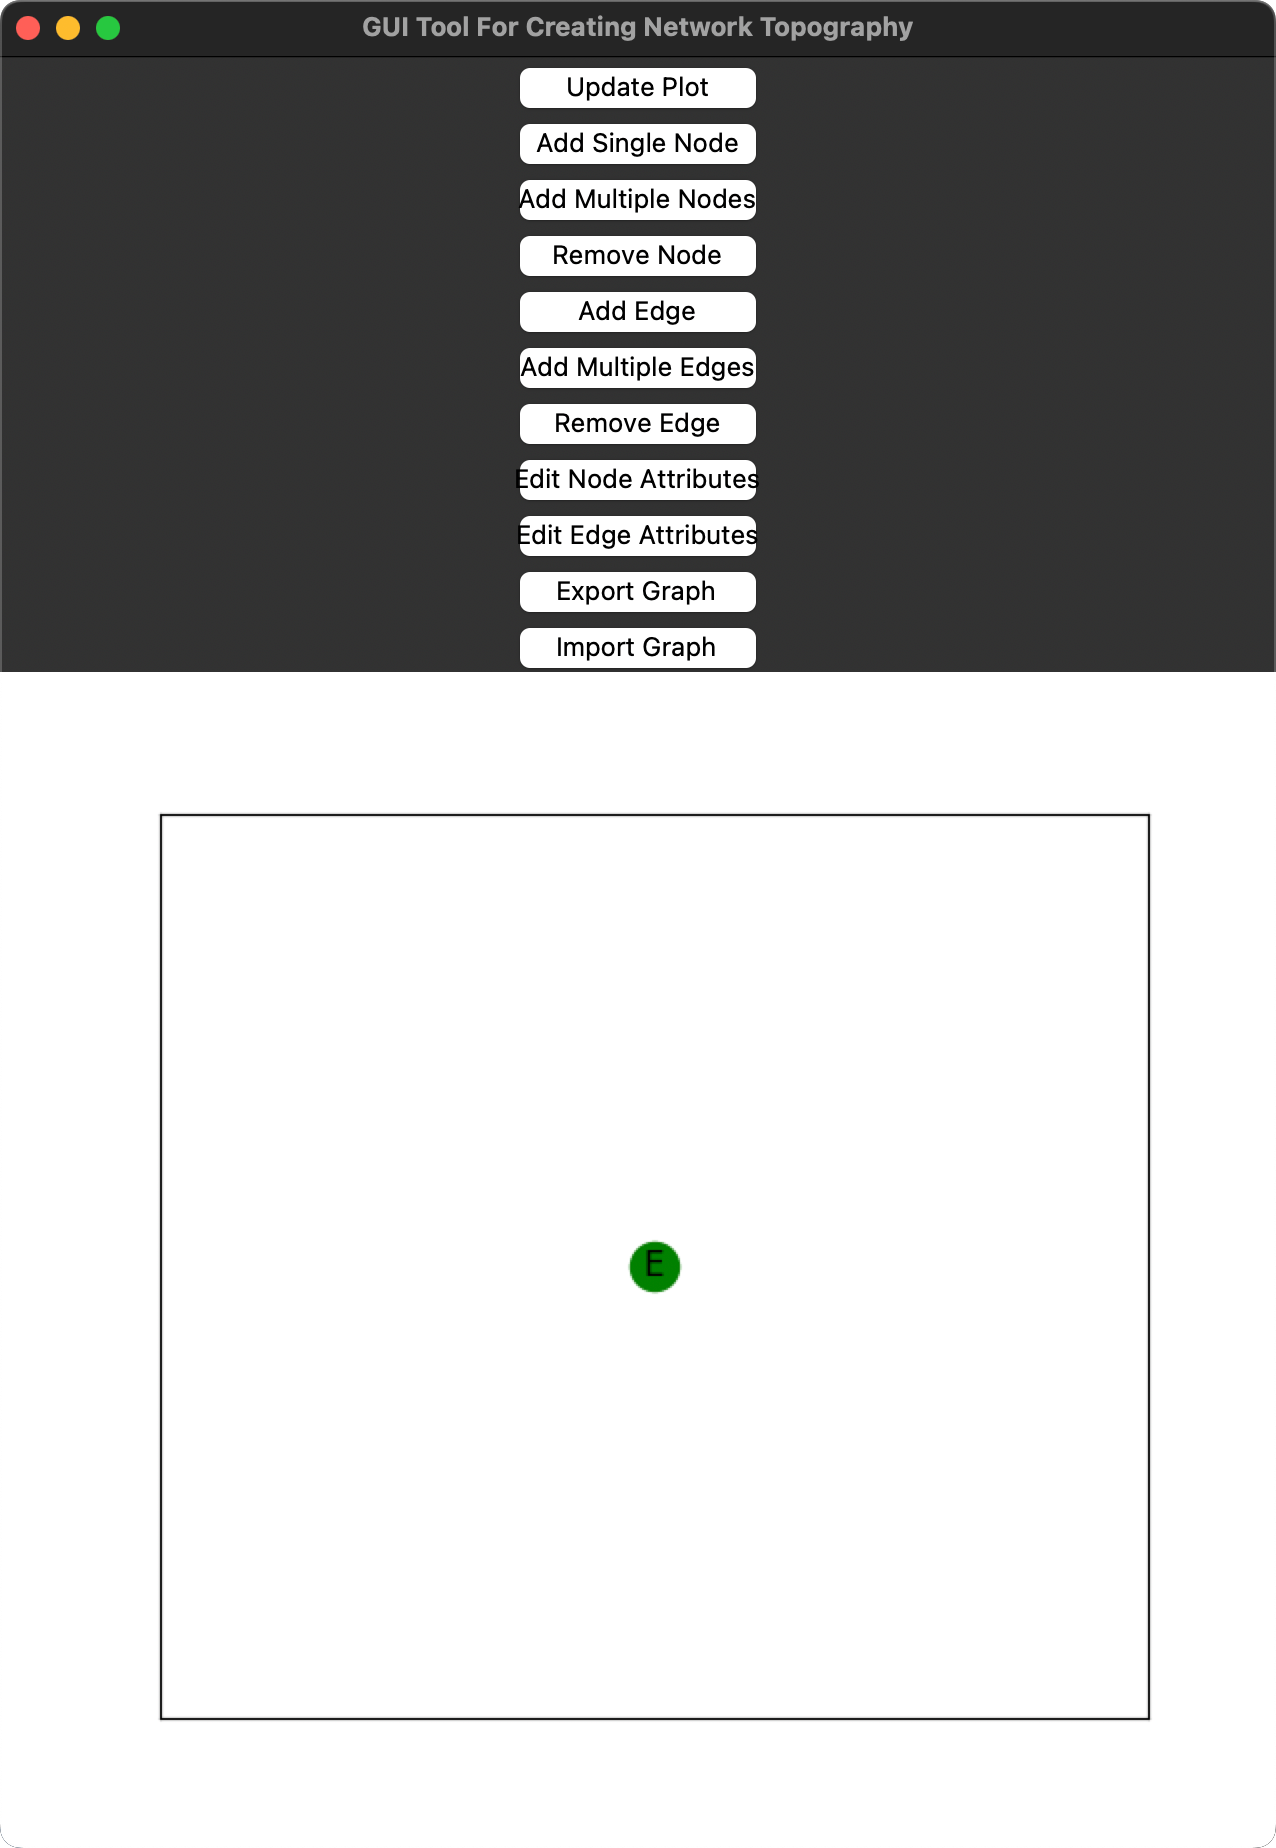
\includegraphics[width=\linewidth]{Screenshots/initial_startup_GUI_tool.png}
        \caption{
            The GUI tool, as seen upon program startup.
        }
        \label{fig:ss:initial_startup_GUI_tool}
    \end{subfigure}
    \begin{subfigure}{0.49\linewidth}
        \centering
        \captionsetup{width=1\linewidth}
        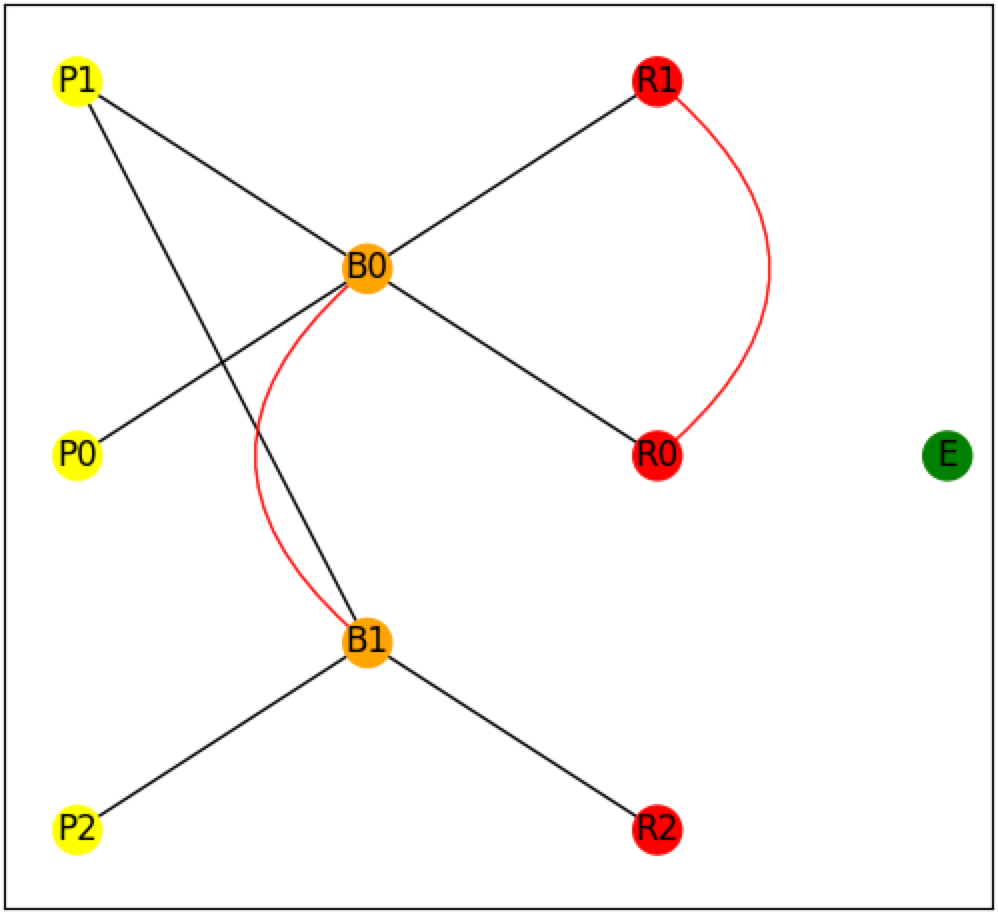
\includegraphics[width=\linewidth]{Screenshots/example_network.png}
        \caption{
            A $1\times1\times1$ and $2\times 2 \times 3$ network. 
        }
        \label{fig:ss:example_network}
    \end{subfigure} 
    \begin{subfigure}{0.49\linewidth}
        \centering
        \captionsetup{width=1\linewidth}
        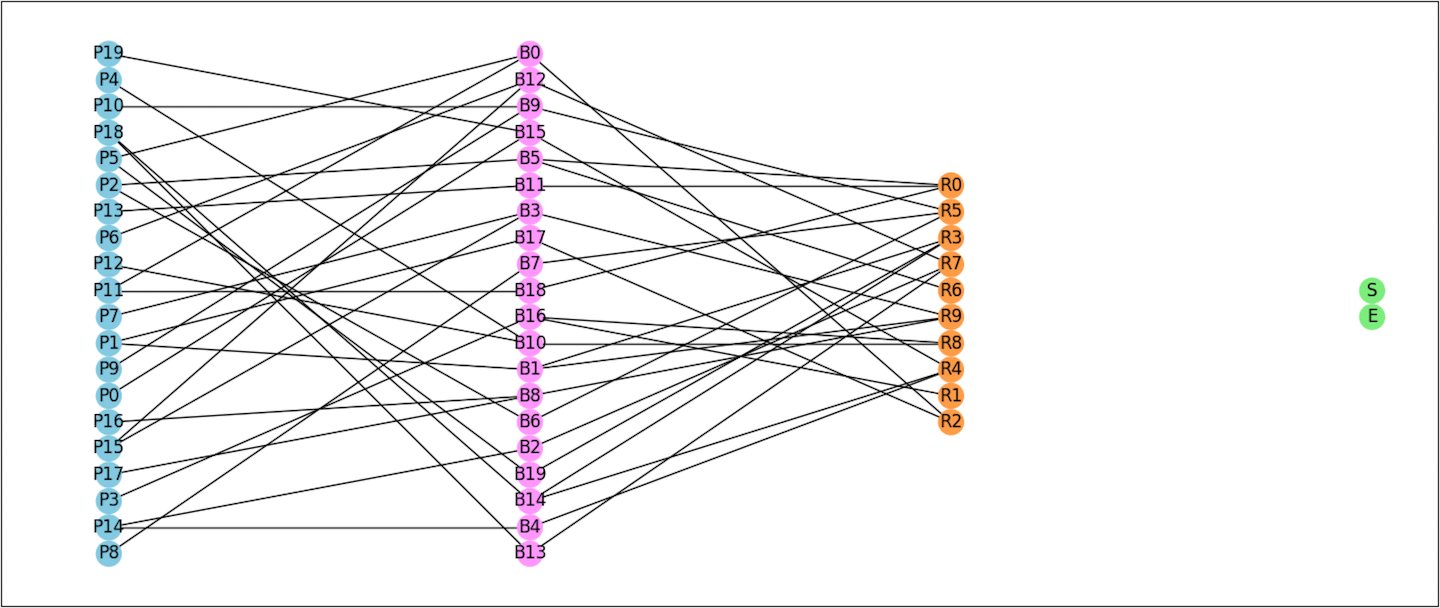
\includegraphics[width=\linewidth]{Screenshots/large_network.png}
        \caption{
            A $20\times20\times10$ network. 
        }
        \label{fig:ss:example_large_network}
    \end{subfigure} 
    \caption{
        This network topography, along with a $1 \times 1 \times 1$ network, will be used in the \Cref{Methods} and \Cref{AER} sections. 
        The parameter values for the networks can be found at \Cref{tab:appendixE:a_good_curve}, \Cref{tab:appendixE:complex_model} and \Cref{tab:appendixE:Sobol_analysis_values}
        Each node represents a phage, bacteria, or resource, with arbitrary interactions occurring between them. 
        Although not shown and used here, edges between the same entity types and self-loops are allowed. 
    }
    \label{fig:ss:GUI_tool_and_network}
 \end{figure}

\subsection{Simulation Framework} % TODO: Rewrite this section
\label{sec:simulation_framework}
The user provides an ODE model and the network topography as input to the framework. 
The simulation framework handles the input, output, collection, and storage of the simulation input and output.
The framework uses SciPy's \cite{virtanenSciPy10Fundamental2020} \textit{solve\_ivp()} numerical solver \cite{ dormandFamilyEmbeddedRungeKutta1980} to simulate the provided ODE equations and calculate the population levels through time.
The user receives two outputs from the framework. 
The first output is an array of time values that the solver used to calculate the population count.
The second output is an array containing the population count at each time step for every entity.

To facilitate more complex model behavior, additional system variables can be added to the simulation.  
An example of this distinction is the difference between uninfected and infected bacteria. 
In the network model, you explicitly create a $3\times 2 \times 3$ network with three phages, two bacteria, and three resources. 
You additionally tell the solver to add $2\cdot M$ additional states that represent the infected states. 
Therefore, the ODE solver would solve for three phages, two uninfected bacteria states, $2\cdot M = 2\cdot 4 = 8$ infected bacteria states, and three resources. 

Adding a resource reservoir to the model would also be straightforward. 
Three extra resource variables would be added to the solver, where the ODE and solver would model the transfer of resources from the reservoir to the simulation environment. 
The provided ODE model must accurately model and transfer resources from $R_{r_{\text{reservoir}}}$ to $R_{r_{\text{chemostat}}}$ correctly. 
The bacteria would only consume from $R_{r_{\text{chemostat}}}$. 

The user's ODE model must accurately represent each (extra) phage, bacterium, and resource and correctly handle changes in states. 

\subsection{Visualization Dashboard}
\label{sec:visualization_framework}
The third part involves analyzing and visualizing the simulation results on an interactive Dash Plotly \cite{DashDocumentationUser} dashboard. 
The user can use a dashboard built using Plotly Dash to interact with the solver and network.
The user can quickly change parameter, environment, and setting values with the dashboard. 
As output, the dashboard displays interactive plots, enabling the user to analyze the system. 

The dashboard enables users to interact with the network, model, and prebuilt visualizations. The dashboard contains three separate sections.
The first section enables the user to edit parameter values and solver settings on the fly, allowing for quick iteration through different conditions and fine-tuning of parameter selection without needing to rebuild the network using the GUI tool.
The second section enables users to visualize how the population count evolves for a given IC and parameter values, allowing them to test the network input quickly.
The final section enables the user to conduct more advanced analyses on the network, for example, by modifying multiple parameter values and visualizing the resulting output. 

\subsubsection{Editing Network and Parameter Values}
\label{sec:editing_network_and_parameter_values}
The editing network and parameter value contain five separate sections.
\paragraph{Initial Condition}
The IC settings panel (\Cref{fig:ss:ds:initial_condition}) allows the user to edit the initial starting values of the entities. 
Each entity type has a table containing the initial population count. 
\paragraph{Vector Data} 
Data stored as a vector, which includes data on the nodes of phages, bacteria, and resources, is displayed in the Vector tab. 
This data is typically associated with node data. 
That would be the washin rate of resources or the bacteria's latent time \Cref{fig:ss:ds:vector}.

\paragraph{Matrix Data}
Data stored as a matrix, typically representing the edges between phages, bacteria, and resources, is stored in the matrix tab, \Cref{fig:ss:ds:matrix}.

\paragraph{Environment and Settings}
The environment data and settings data also have their own tab, \Cref{fig:ss:ds:environment} and \Cref{fig:ss:ds:settings}, respectively. 
The data stored in the environment act as global variables, like the pH of the system or the constant washout rate $\omega^o$. 
The settings node contains the solver and simulation settings, including the simulation length and minimum time step. 

\begin{figure}[h!]
    \centering
    \begin{subfigure}{0.49\linewidth}
        \centering
        \captionsetup{width=1\linewidth}
        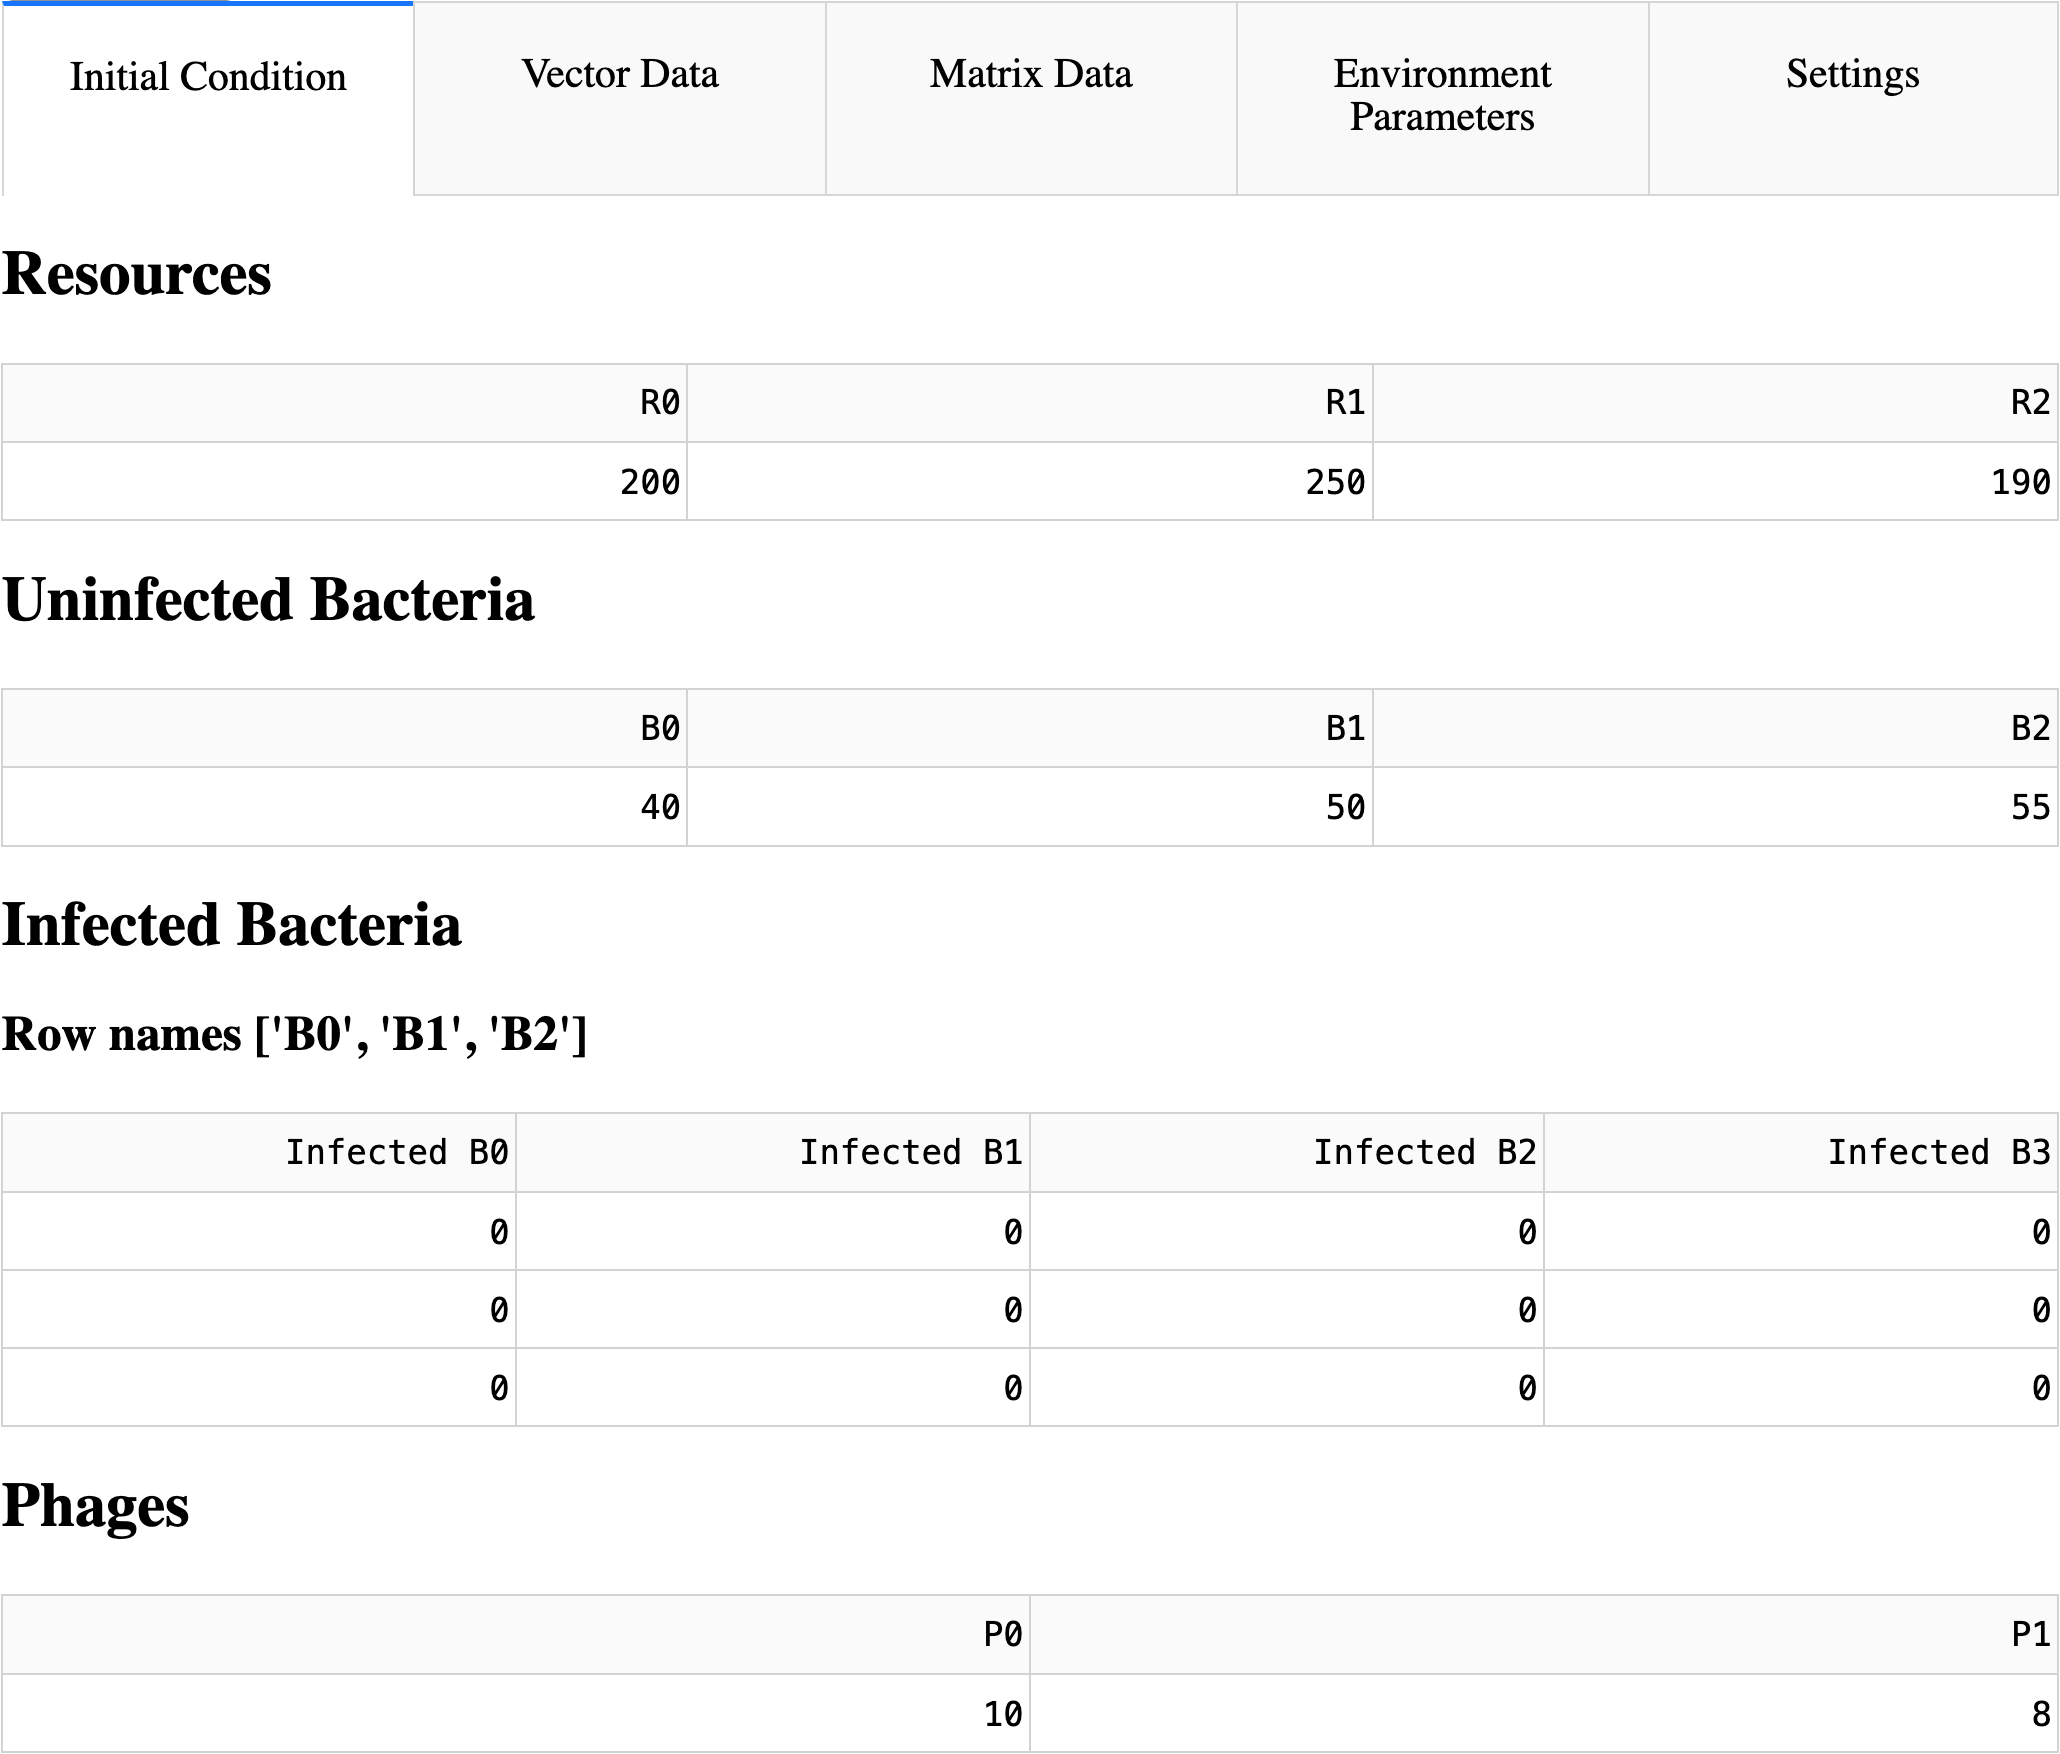
\includegraphics[width=\linewidth]{Screenshots/DashboardSettings/initial_condition_settings.png}
        \caption{
            The tab where users can edit the ICs of the entities.
        }
        \label{fig:ss:ds:initial_condition}
    \end{subfigure}
    \hfill
    \begin{subfigure}{0.49\linewidth}
        \centering
        \captionsetup{width=1\linewidth}
        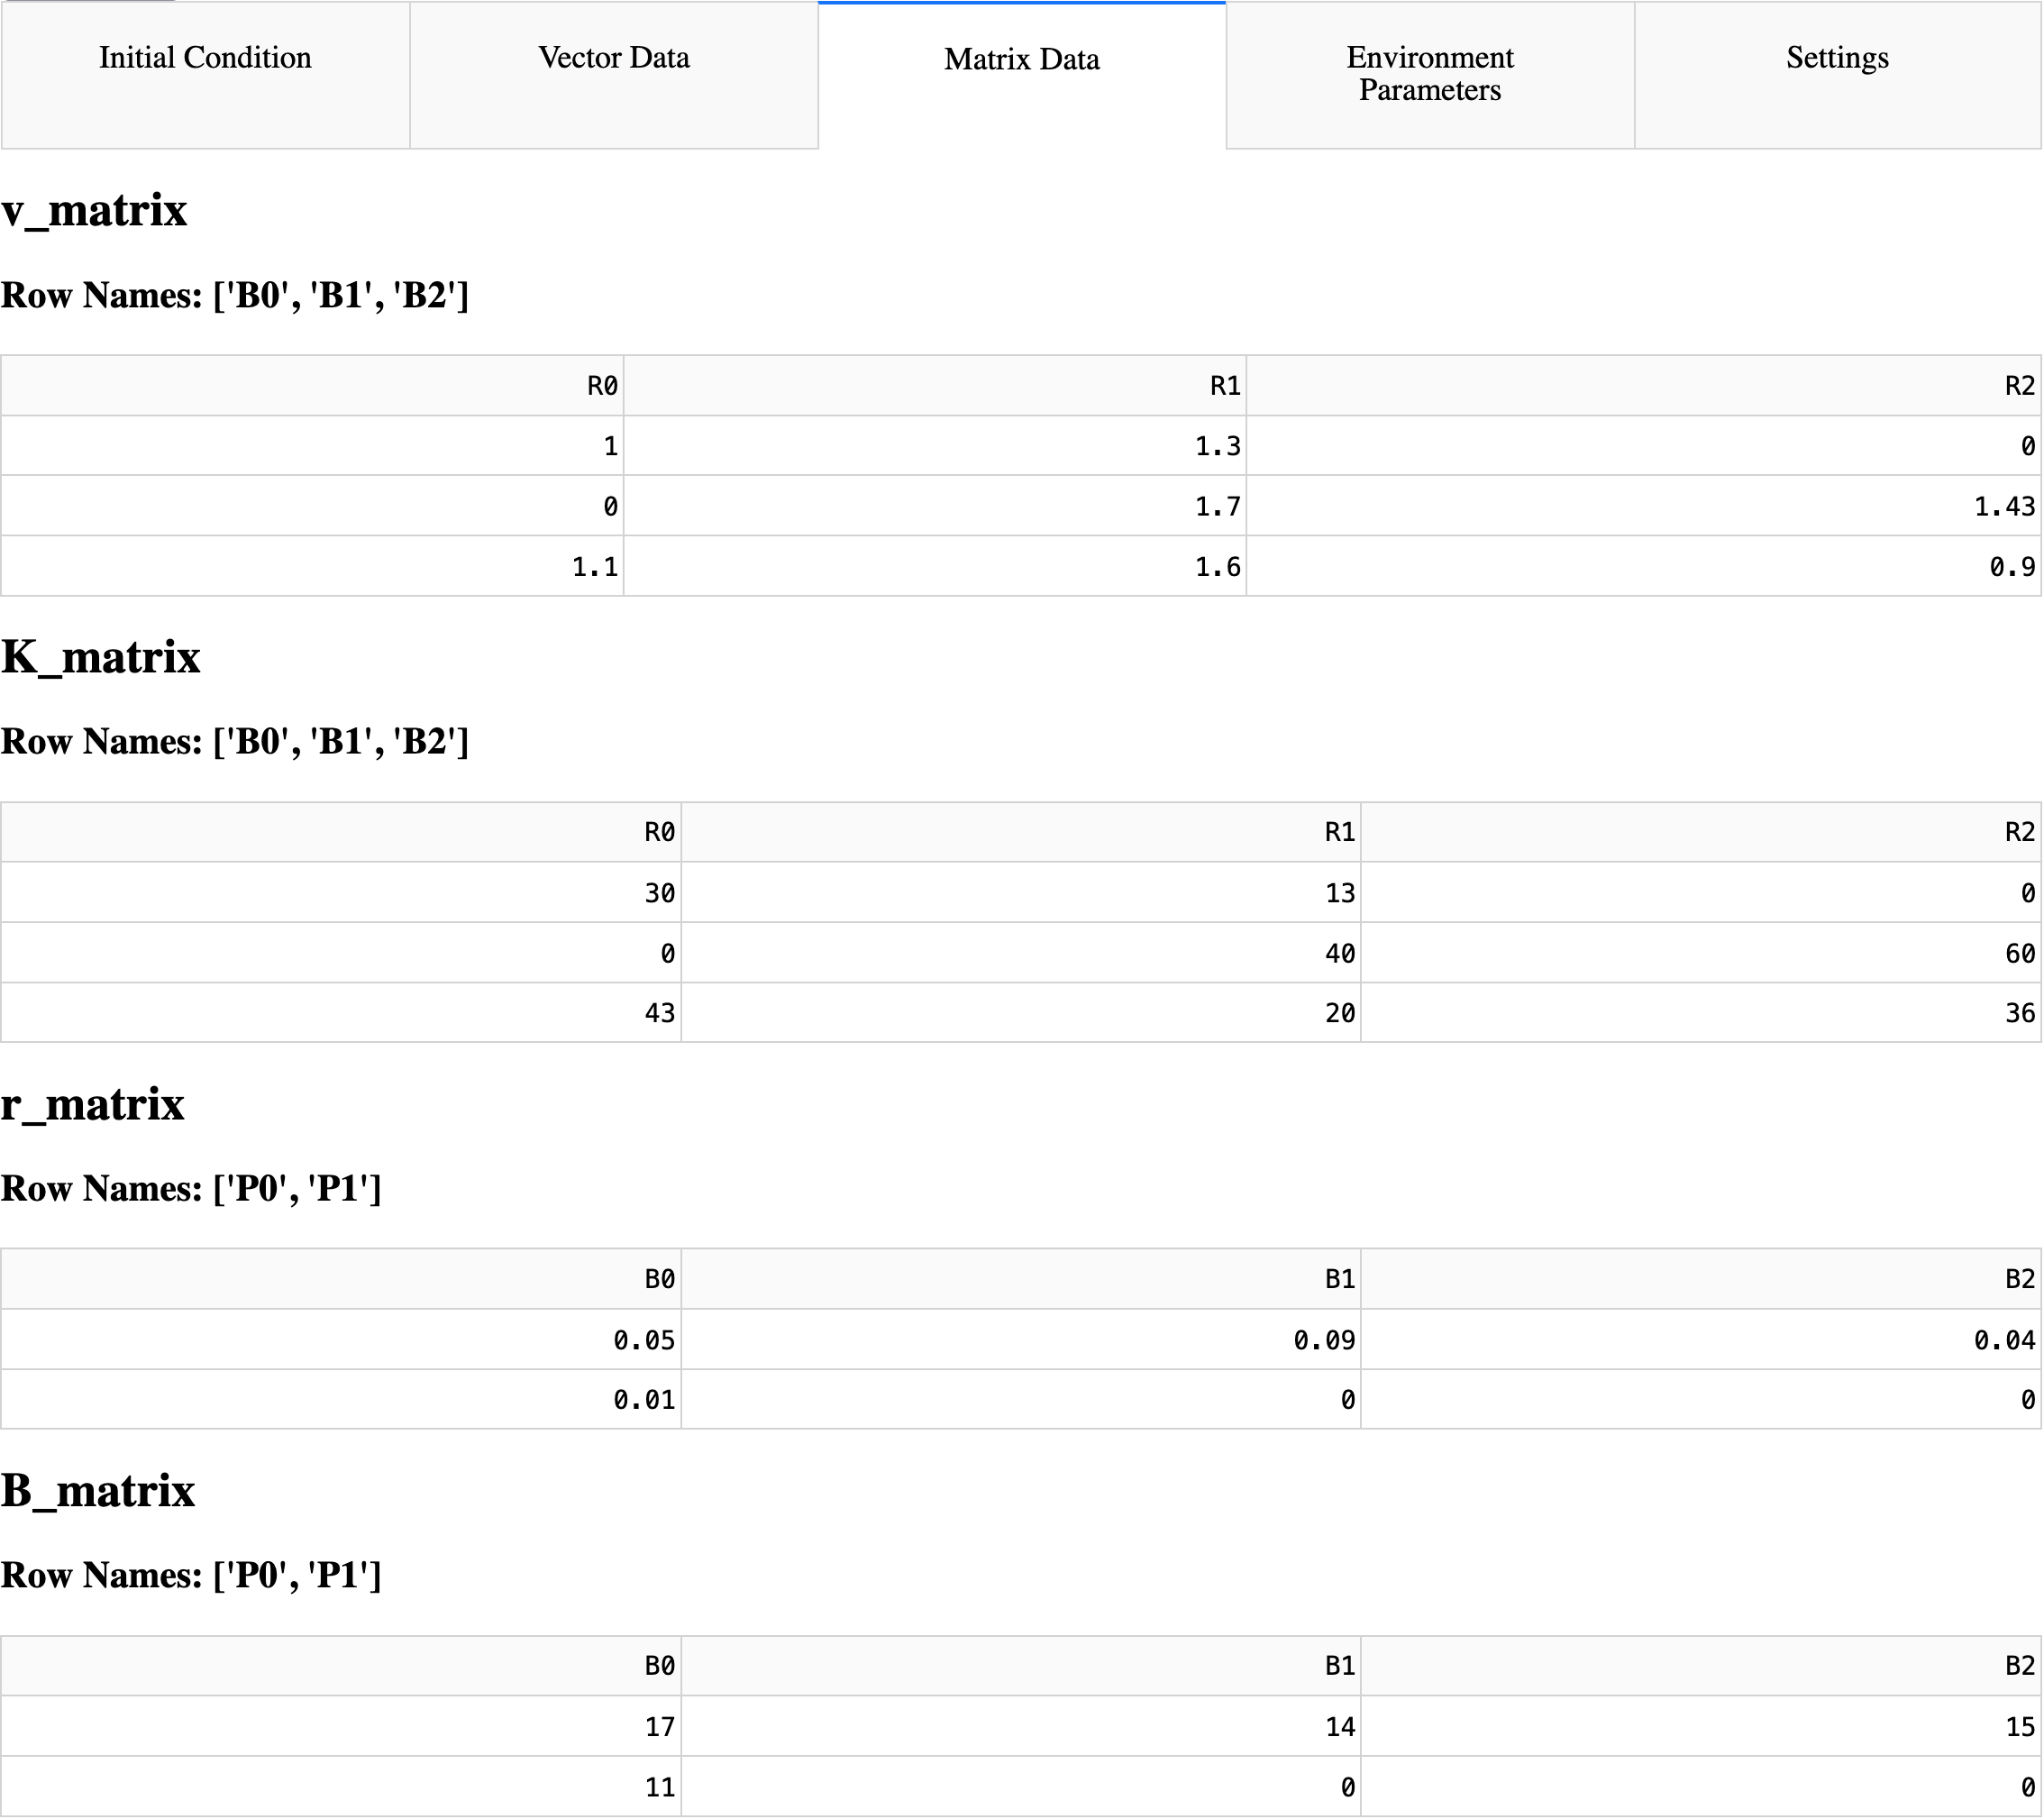
\includegraphics[width=\linewidth]{Screenshots/DashboardSettings/initial_matrix_settings.png}
        \caption{
            The tab where the user can edit the matrix attribute values. 
        }
        \label{fig:ss:ds:matrix}
    \end{subfigure}
    \hfill
    \begin{subfigure}{0.49\linewidth}
        \centering
        \captionsetup{width=1\linewidth}
        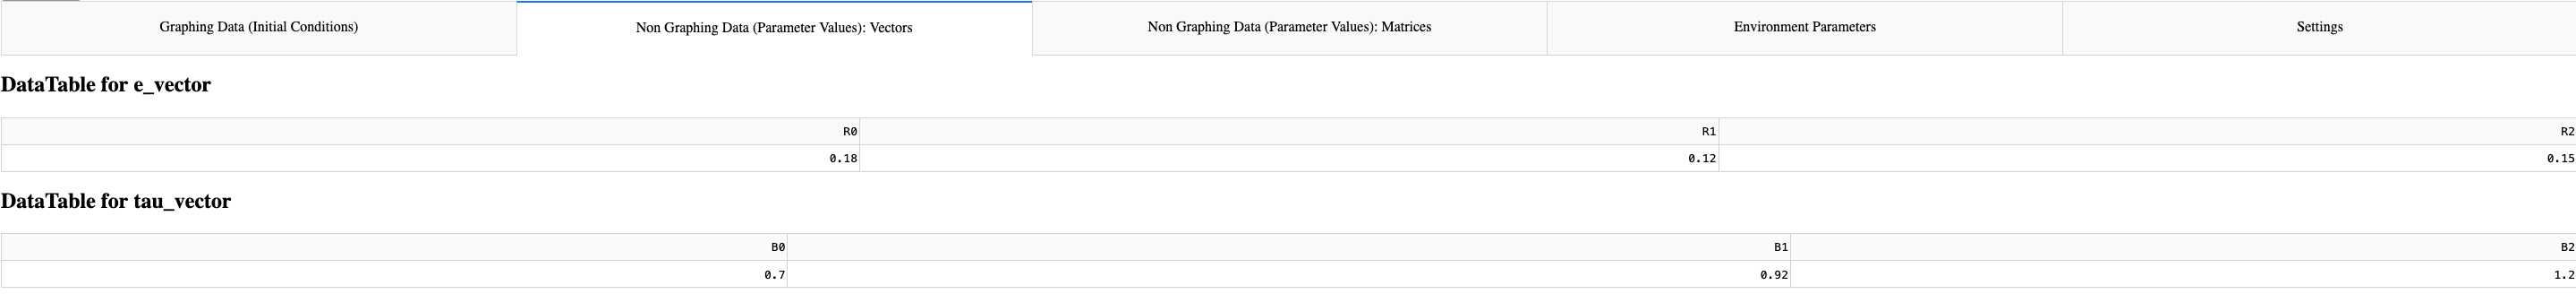
\includegraphics[width=\linewidth]{Screenshots/DashboardSettings/initial_vector_settings.png}
        \caption{
            The tab where users can edit vector attribute values.
        }
        \label{fig:ss:ds:vector}
    \end{subfigure}
    \hfill
    \begin{subfigure}{0.49\linewidth}
        \centering
        \captionsetup{width=1\linewidth}
        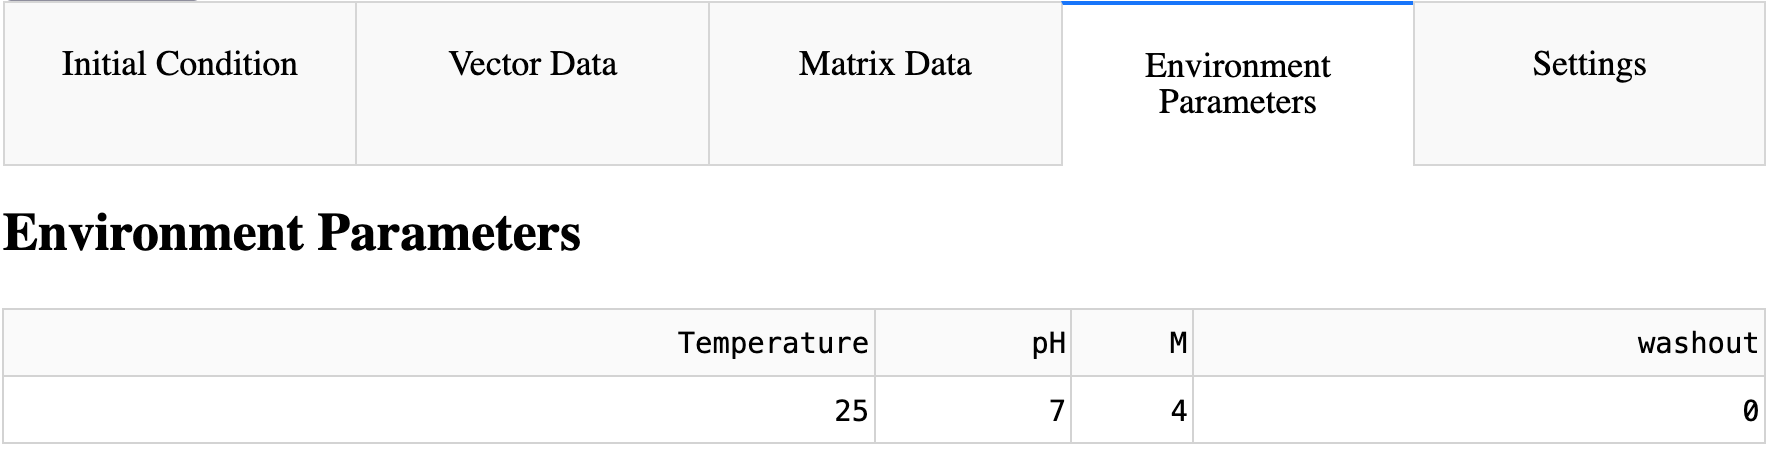
\includegraphics[width=\linewidth]{Screenshots/DashboardSettings/initial_environment_settings.png}
        \caption{
            The tab where users can edit environment values. 
        }
        \label{fig:ss:ds:environment}
    \end{subfigure}
    \hfill
    \begin{subfigure}{0.49\linewidth}
        \centering
        \captionsetup{width=1\linewidth}
        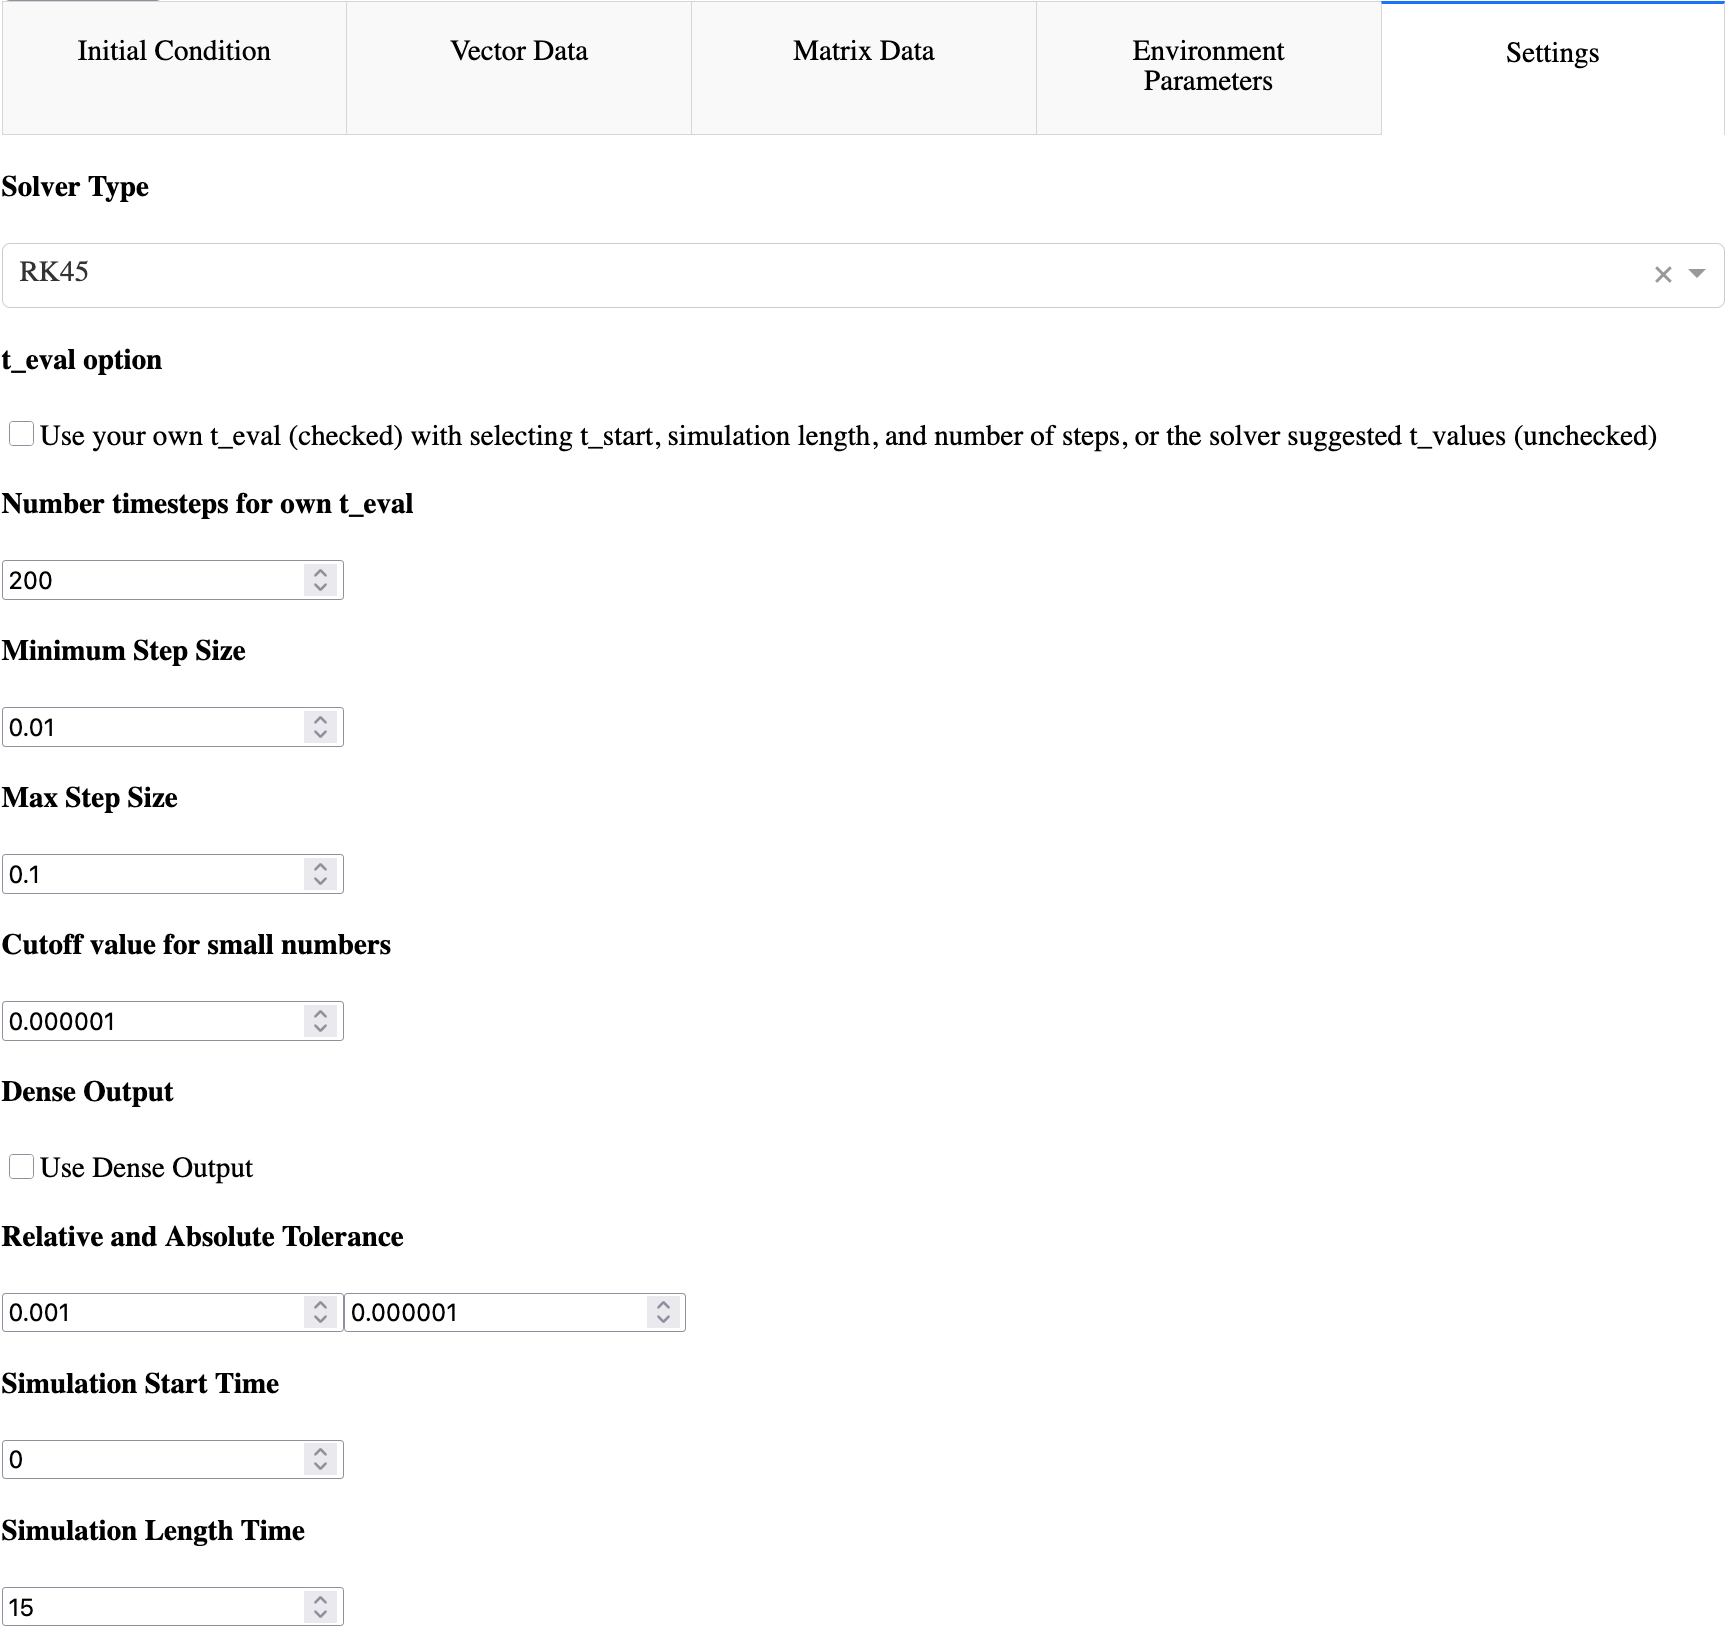
\includegraphics[width=\linewidth]{Screenshots/DashboardSettings/initial_settings_settings.png}
        \caption{
            The tab where a user can edit the settings of the solver and simulation. 
        }
        \label{fig:ss:ds:settings}
    \end{subfigure}
    \caption{The tabs where the user can edit the various parameter values and control the simulation parameters}
 \end{figure}

\subsubsection{Visualization and Analysis}
In the analysis section, the user can run different analysis methods to gain a greater understanding of the model.
For simplicity, the visualizations on the dashboard only support a $1 \times 1\times 1$ model. 
This makes it easier for the user to analyze the system. 
The goal of the dashboard is to investigate a simple system in order to gain a deeper understanding of the system. 
The next step is to simulate more complex models using the Ultimate Analysis section, where you implement your own visualizations. 
There are five prebuilt visualizations, which are described below. 
These five visualizations are called serial transfer, parameter analysis, initial value analysis, phase portrait, and Sobol analysis. 
The aim of these visualizations is to investigate how a simple system responds to varying inputs before moving on to more complex models. 

After the user has a deeper understanding of the system, they can run and download custom simulations to create their own custom visualizations in the Ultimate Analysis section. 
The saved simulation data is stored as a \textit{.parquet} file, a tabular-like data format. 
Dask can query the simulation data, allowing users to find specific simulation results. 
Parquet with Dask offers superior performance and data storage solutions that Pandas does not offer.

\paragraph{Serial Transfer}
\label{sec:serial_transfer}
On the dashboard, a user can select the dilution factor, which divides the phage, bacteria, and resource population count by that number (\Cref{fig:ss:av:serial_transfer_settings}).
Then, the program takes the IC values defined in \Cref{sec:editing_network_and_parameter_values} and adds those values to the respective entity. 

As an example, if the simulation ended with 3500 phages, 100 (uninfected) bacteria, and 50 resources, the dilution factor is 10, and the user wants to add 350 new bacteria and 130 new resources for the following simulation, the new starting condition for the following simulation would be $\frac{3500}{10} = 350$ phages, $\frac{100}{10} + 350 = 660$ bacteria, and $\frac{50}{10} + 130 = 135$ resources.

As output, ST will display how the population evolves, as well as the final population value at the end of each serial transfer run. 
An example output is shown in \Cref{fig:ss:av:serial_transfer_run}.

\begin{figure}[h!]
    \centering
    \begin{subfigure}{0.49\linewidth}
        \centering
        \captionsetup{width=1\linewidth}
        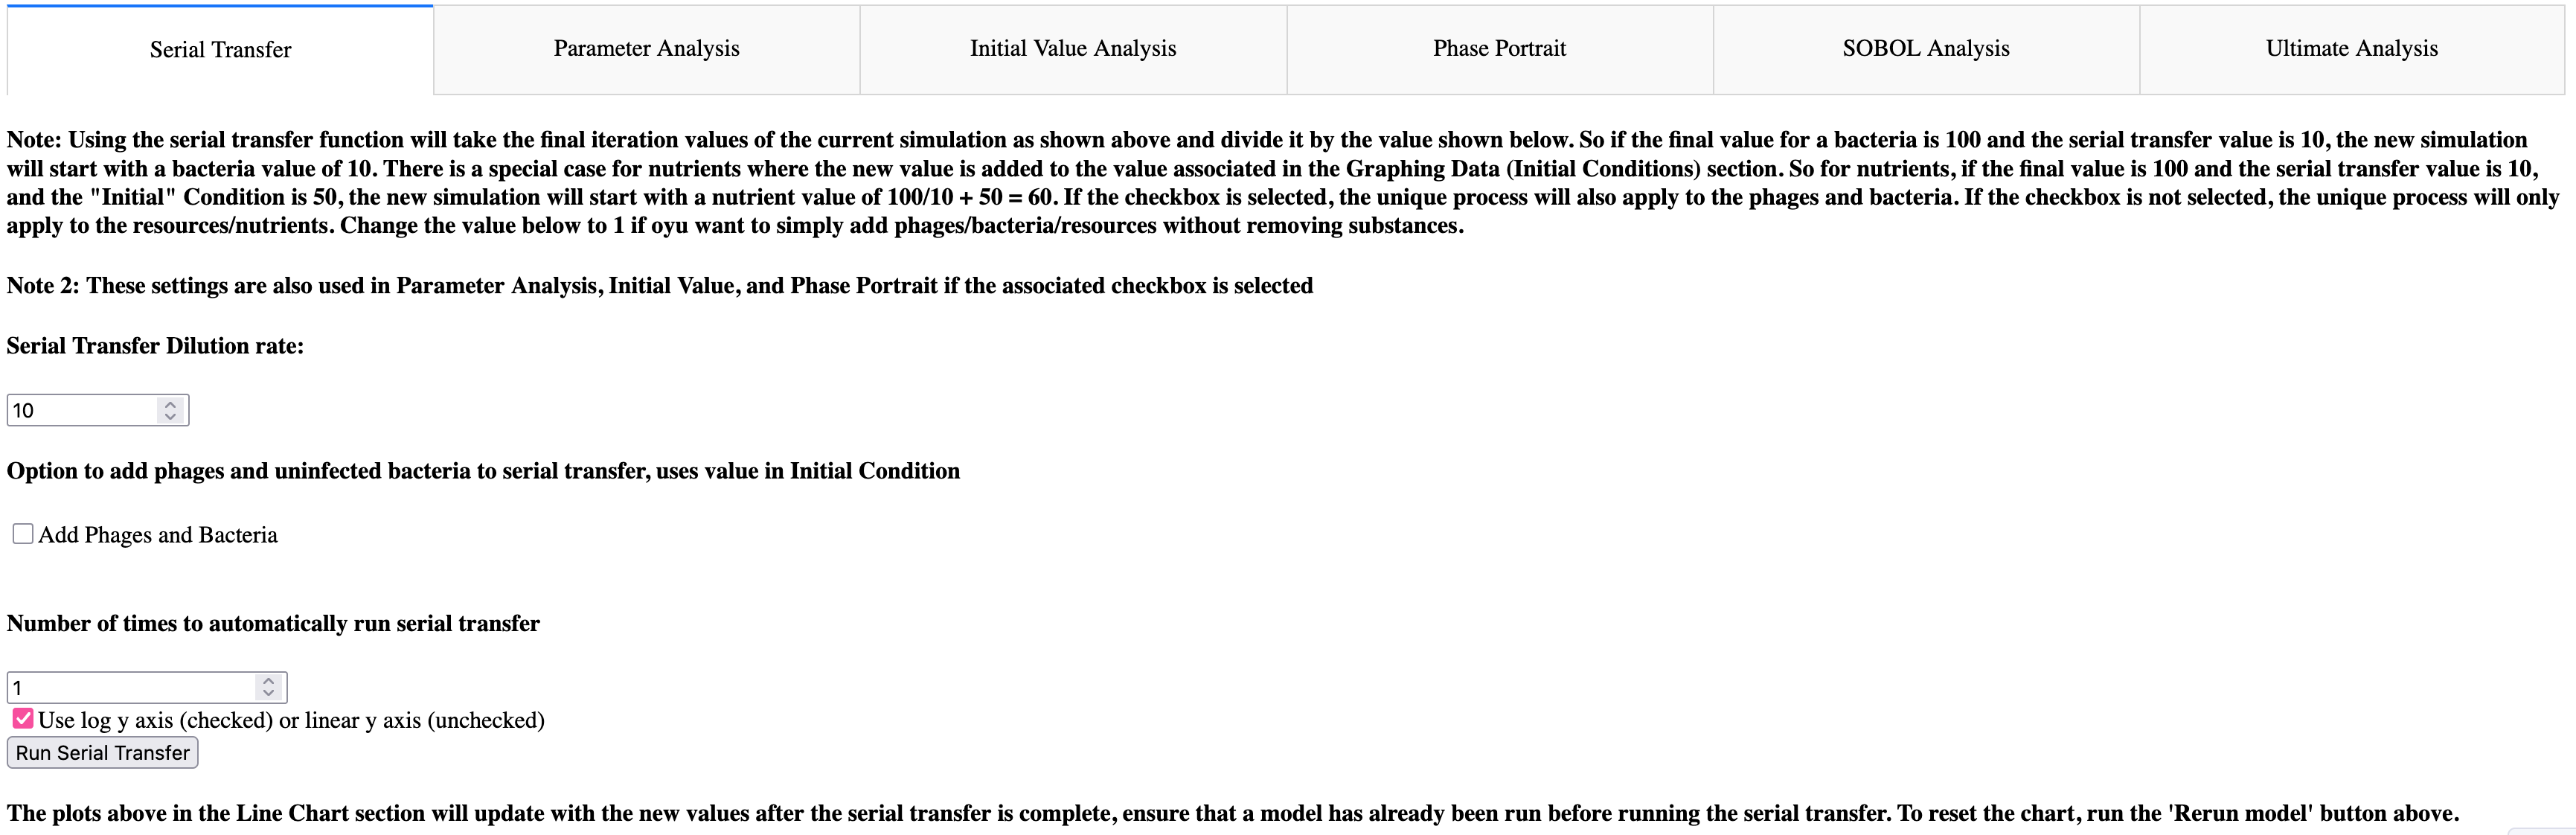
\includegraphics[width=\linewidth]{Screenshots/AdvancedVisualization/serial_transfer_settings.png}
        \caption{
            The section where the user can set up the ST.
        }
        \label{fig:ss:av:serial_transfer_settings}
    \end{subfigure}
    \hfill
    \begin{subfigure}{0.49\linewidth}
        \centering
        \captionsetup{width=1\linewidth}
        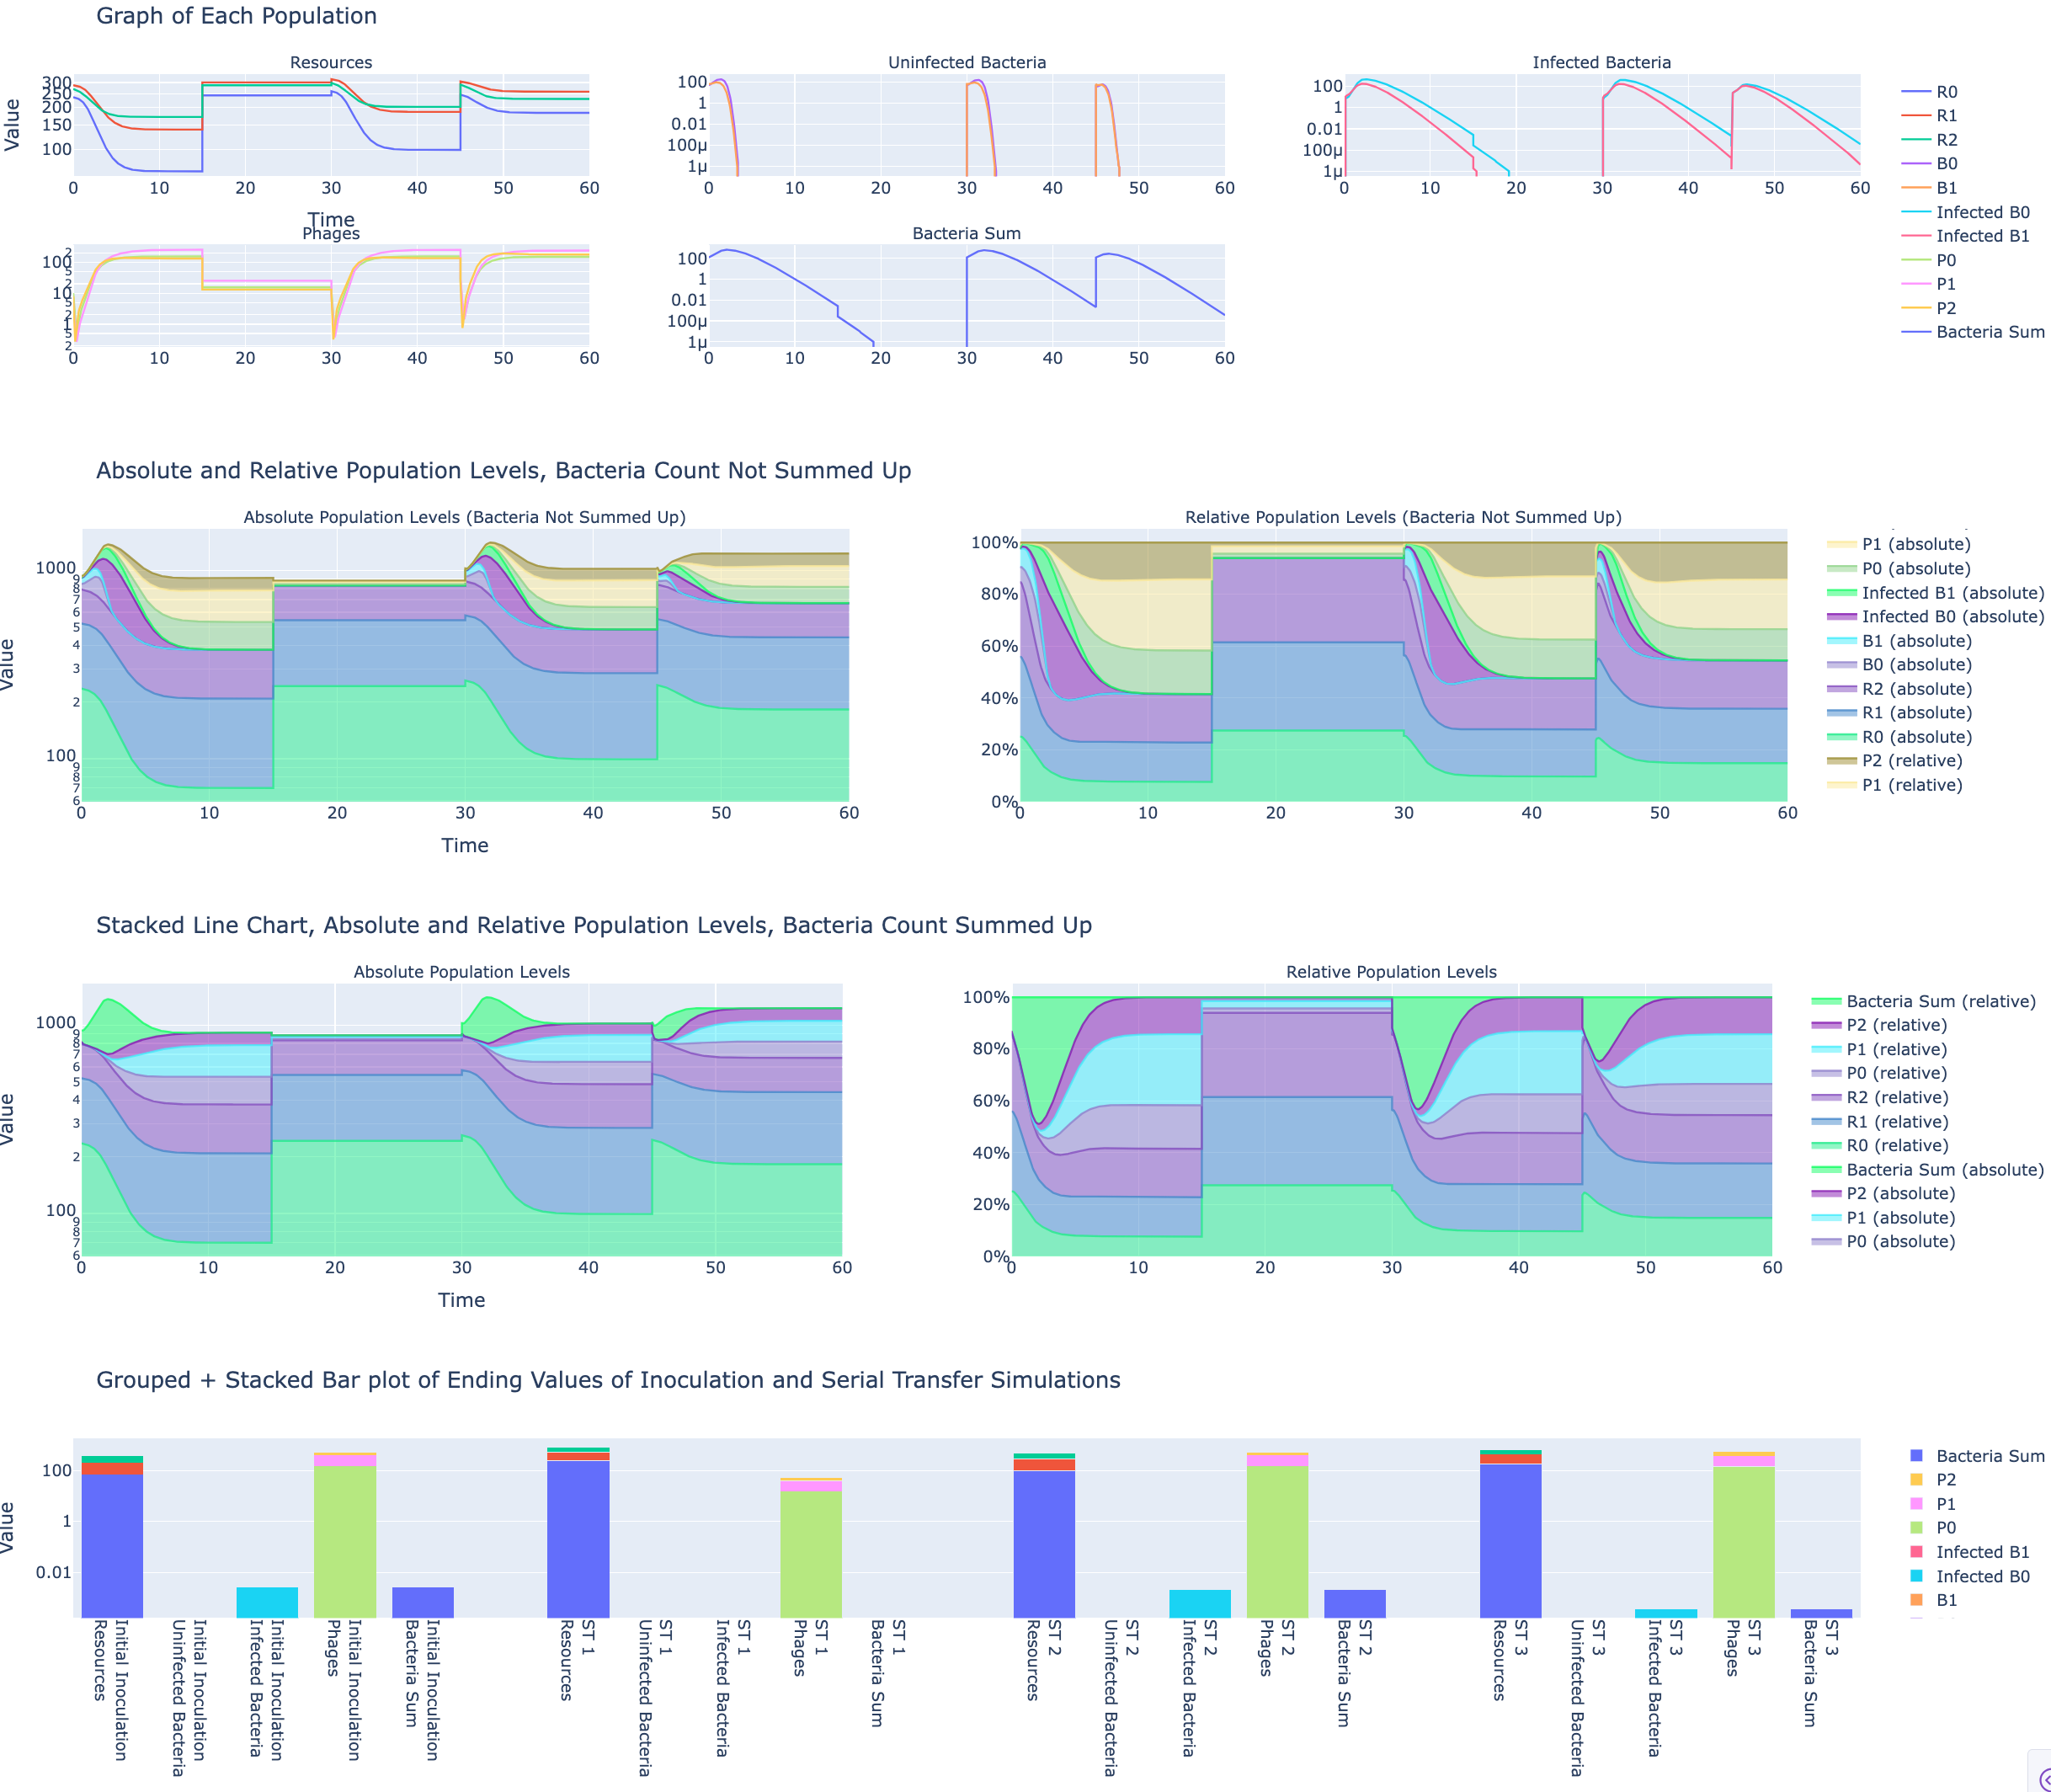
\includegraphics[width=\linewidth]{Screenshots/AdvancedVisualization/serial_transfer_run.png}
        \caption{
            The ST output plots. 
        }
        \label{fig:ss:av:serial_transfer_run}
    \end{subfigure}
    \caption{The ST settings and output.}
\end{figure}

\paragraph{Parameter Analysis}
\label{sec:parameter_analysis}
The Parameter Analysis (PA) settings tab, as shown in \Cref{fig:ss:av:parameter_analysis_settings}, allows the user to select two parameters and individually run the model with varying input values.
The values that can be tested and changed include all IC values, vector and matrix data, and environmental data.
As input, the user can select two parameters of choice.
The user can manually choose which parameter values they want to test or test a range of values equally spaced by selecting the number of values to test.
Finally, the user can optionally run a ST, where the ST uses the settings found on the ST tab. 

\Cref{fig:ss:av:parameter_analysis_run} shows the heatmap that the user can expect, one heatmap for each entity type.
Each heatmap cell represents the input of two unique parameter values and shows the population count for that parameter run at the time indicated by the slider. 
As the user slides the slider, the value inside the cell updates to correspond with the selected time. 
Note that the heatmap color range resets for each heatmap, so similar colors across heatmaps and across time will not correspond to the same values.

\begin{figure}[h!]
    \centering
    \begin{subfigure}{0.49\linewidth}
        \centering
        \captionsetup{width=1\linewidth}
        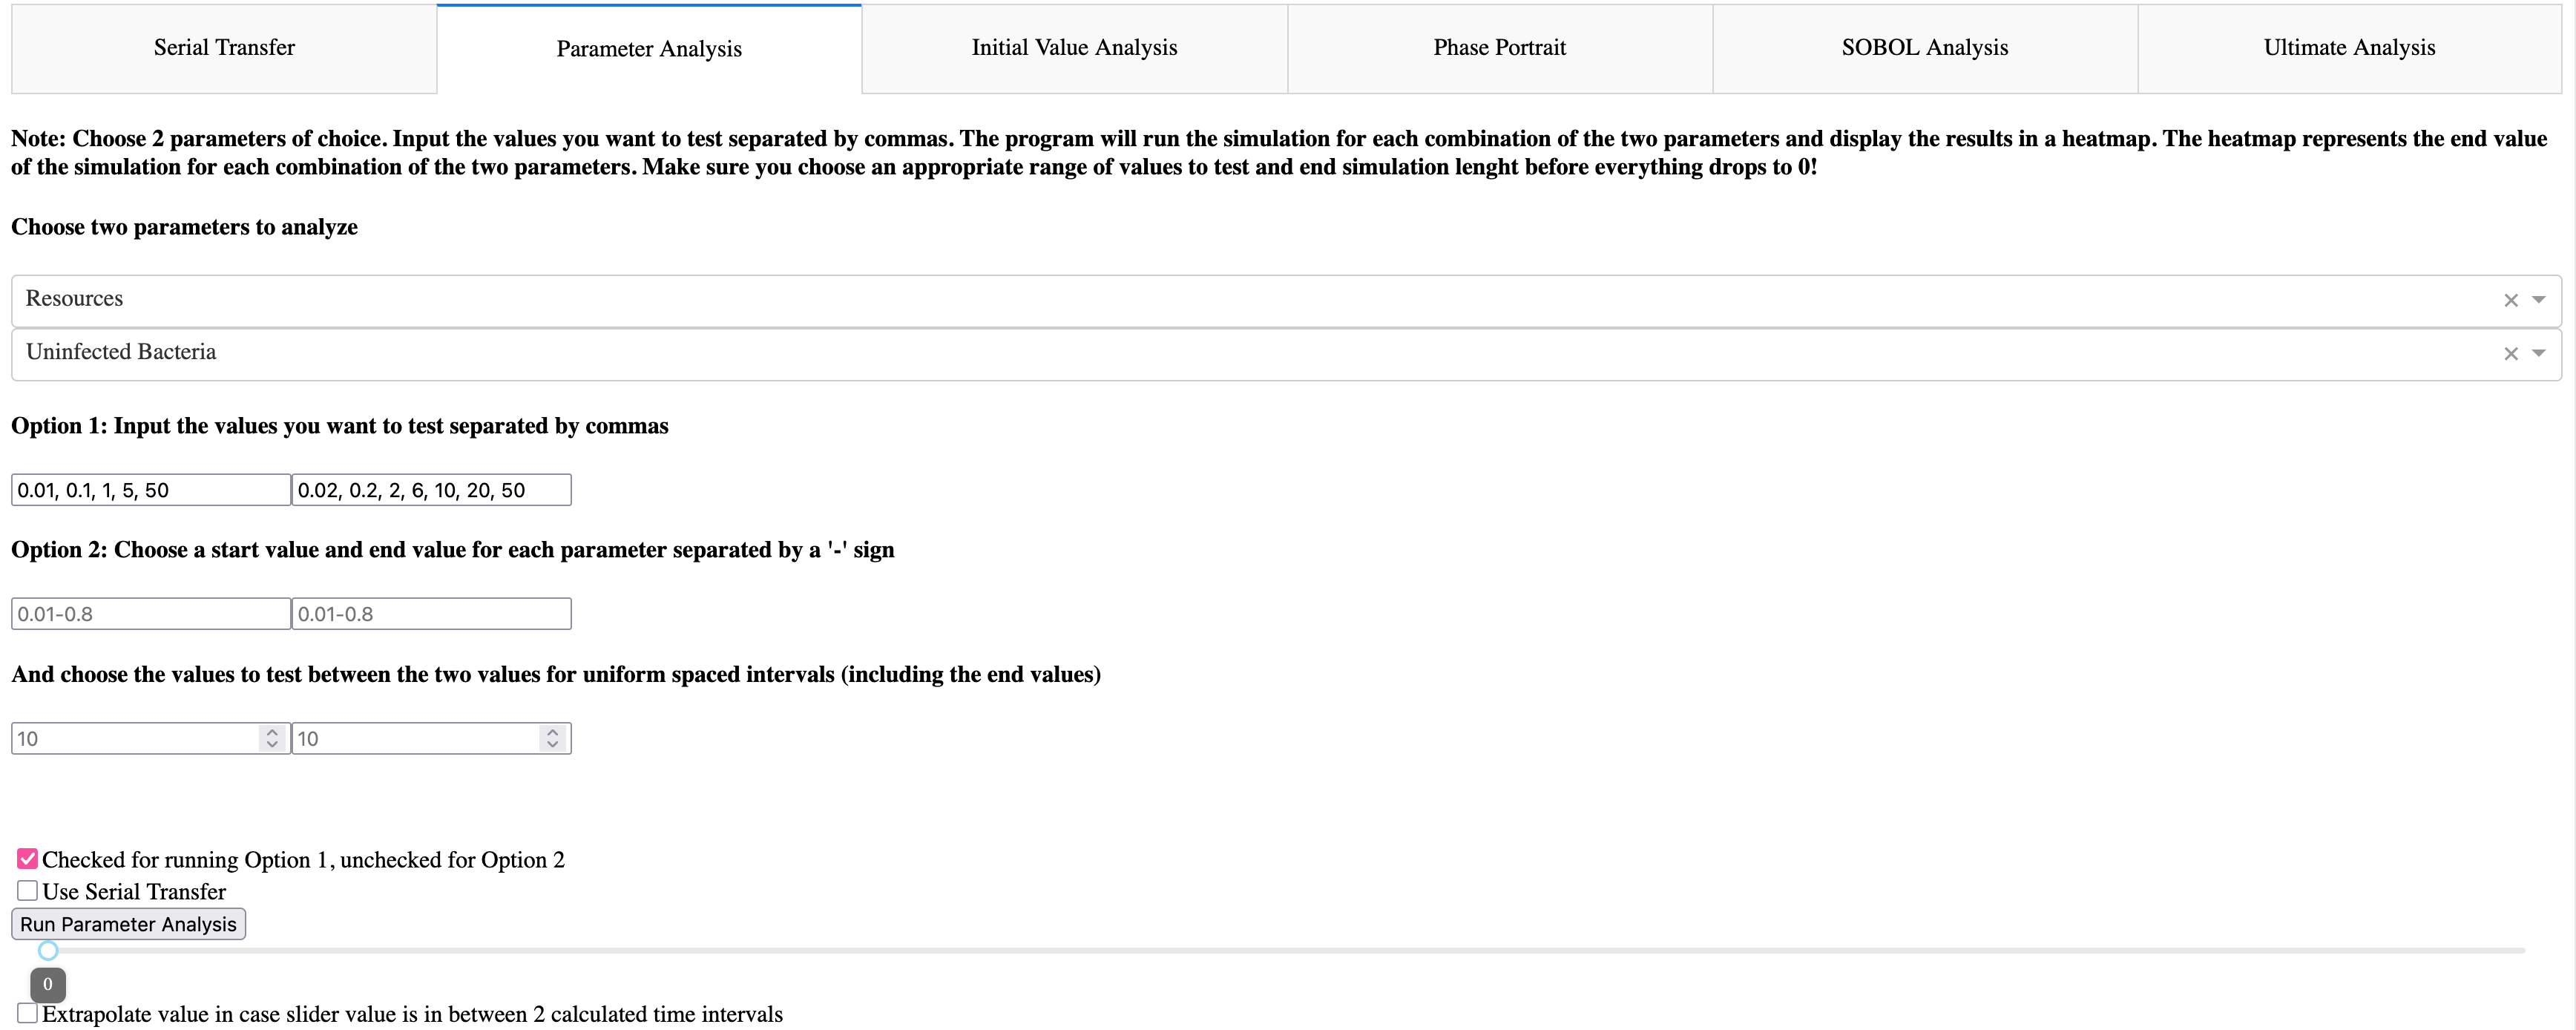
\includegraphics[width=\linewidth]{Screenshots/AdvancedVisualization/parameter_analysis_settings.png}
        \caption{
            The available PA settings. 
        }
        \label{fig:ss:av:parameter_analysis_settings}
    \end{subfigure}
    \hfill
    \begin{subfigure}{0.49\linewidth}
        \centering
        \captionsetup{width=1\linewidth}
        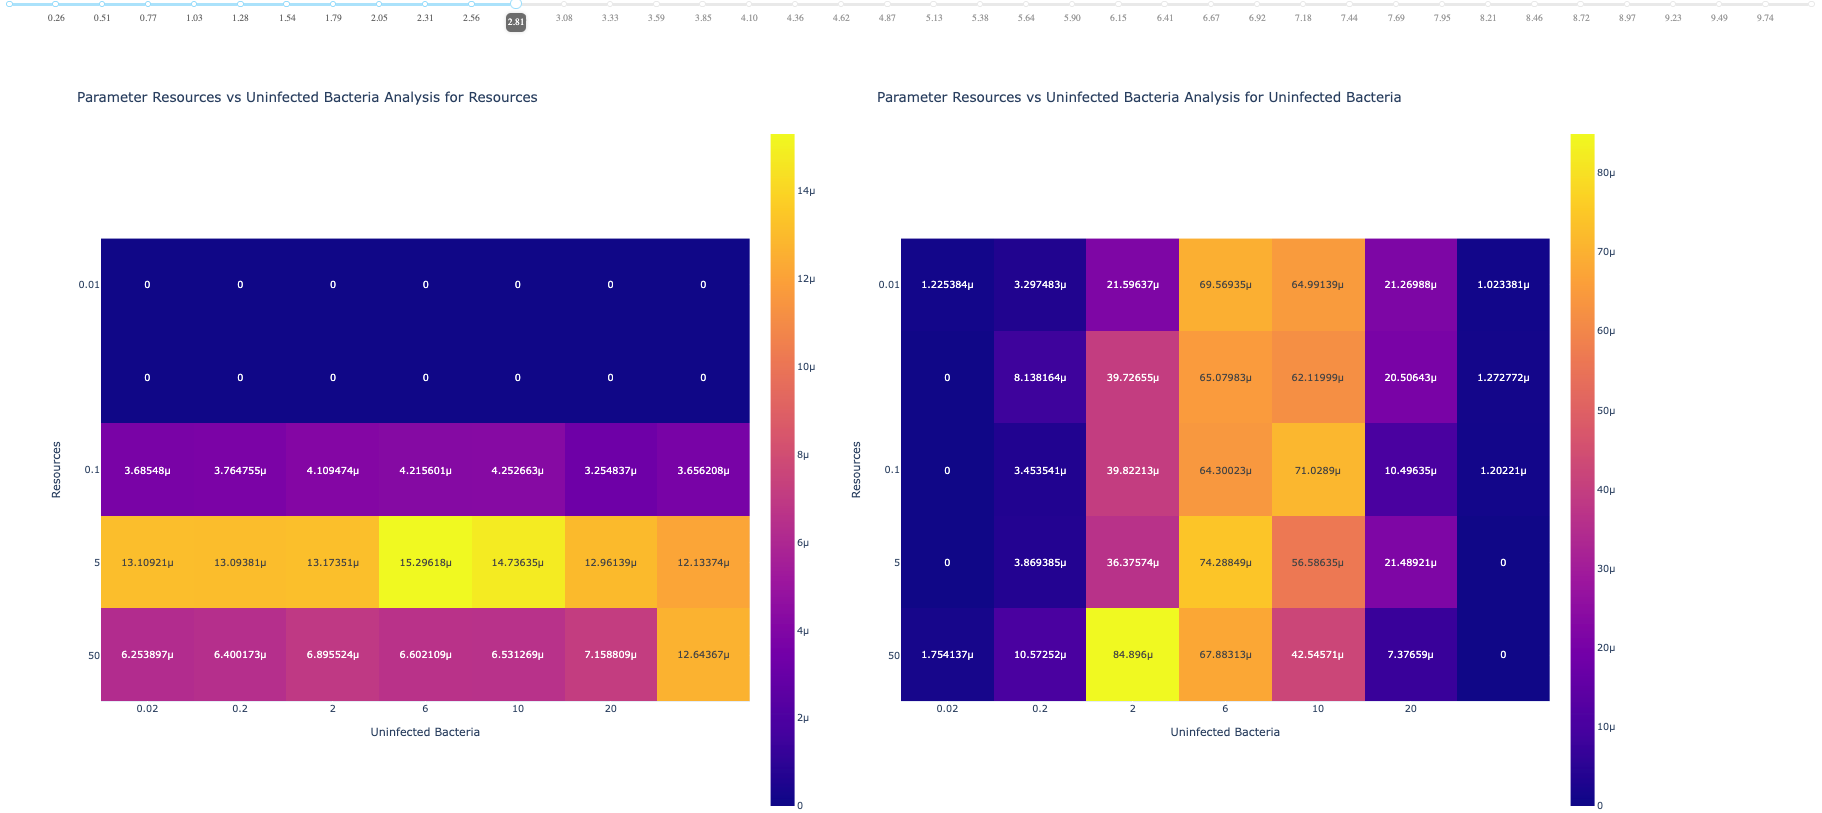
\includegraphics[width=\linewidth]{Screenshots/AdvancedVisualization/parameter_analysis_run.png}
        \caption{
            The expected PA output. 
            The left figure is the PA output for the resource value at $t=2.81$ for different initial uninfected bacteria and initial resource concentration, while the right figure shows the value of the uninfected population at $t=2.81$. 
        }
        \label{fig:ss:av:parameter_analysis_run}
    \end{subfigure}
    \caption{The PA settings and output.}
\end{figure}

\paragraph{Initial Value Analysis}
\label{sec:initial_value_analysis}
The initial value analysis (IVA) settings tab, as shown in \Cref{fig:ss:av:initial_value_analysis_settings}, allows the user to select a single parameter and adjust its value over a range of values, visualizing how a change in parameter value affects the population count of the entities.

\Cref{fig:ss:av:initial_value_analysis_run} shows the plots that the user receives.
For each entity type, three plots are created.
The left plot shows the population count through time, one line for each parameter value submitted.
The middle plot takes each run and calculates the “percentage from the max value” (default value of $0.95 \rightarrow 95\%$) reached from the peak.
In short, the 95\% rule identifies the maximum value reached during the simulation, then calculates 95\% of that maximum. 
It determines the time point at which this 95\% threshold is first reached.
See \Cref{sec:appendixF:why_95} for more information on what the 95\% rule is. 
This value is considered the time of peak and is used to address some issues that can arise when the population plateaus or continues to rise.
For example, suppose the phage population starts to plateau early in the simulation. 
In that case, the program can calculate that the “peak” of the phage population happened at the beginning of the simulation. 

The initial value is placed on the x-axis, while the time of peak value appears on the y-axis. 
Using the plotted data, a linear or log fit can be made.
In Figure 1 of \citet{mullaExtremeDiversityPhage2024} (see \Cref{fig:sourced:Mulla}), the authors vary the initial bacterial concentration and measure the time until bacterial collapse. 
The initial concentration and corresponding collapse time are plotted on a logarithmic x-axis, with a linear regression fitted to the log-transformed data.
The observed logarithmic decrease suggests that the phage kinetics is adsorption-limited. 
\Cref{fig:created:initial_value_analysis_UB_50_500_a_good_plot_2} replicates this graph. 

Using the IVA tool can help understand how a change in parameter value affects the time at which the population count reaches a maximum.
The slope, intercept, and $R^2$ value are stored and saved in the third plot, a bar chart with an editable name. 
For every rerun of the IVA, the bar chart stores the slope, intercept, and $R^2$ value and displays the linear regression next to previous runs. 
When executed with multiple parameters, this enables comparison of high-level results across various parameters and experimental conditions.

\begin{figure}[h!]
    \centering
    \begin{subfigure}{0.49\linewidth}
        \centering
        \captionsetup{width=1\linewidth}
        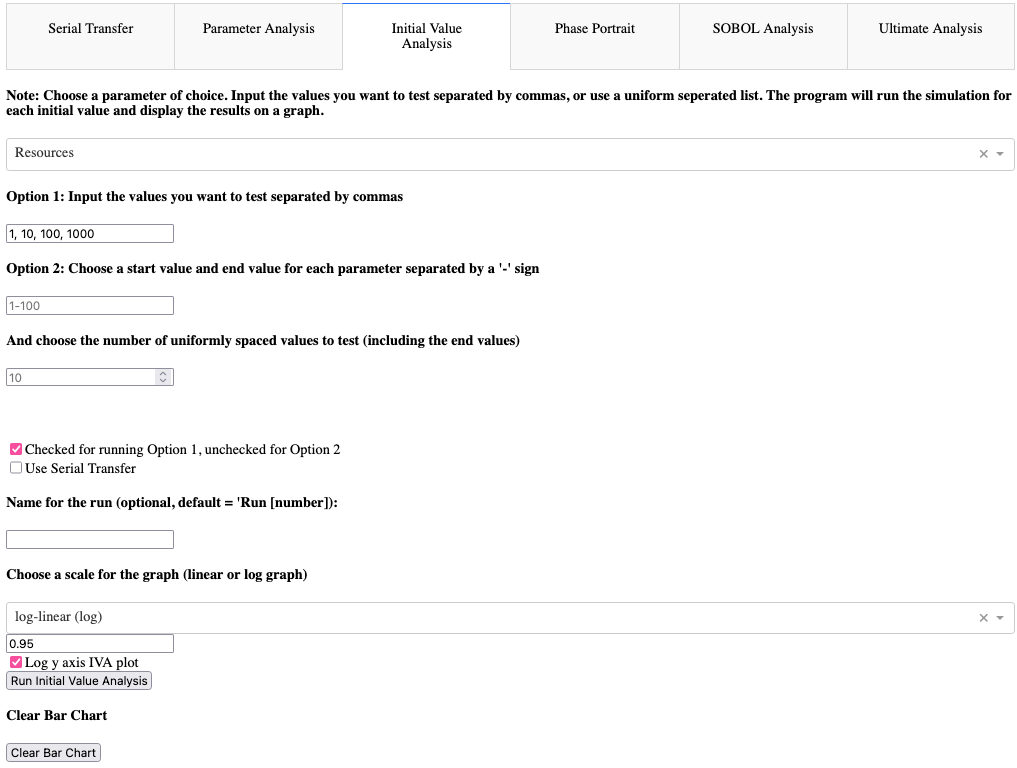
\includegraphics[width=\linewidth]{Screenshots/AdvancedVisualization/initial_value_analysis_settings.png}
        \caption{
            The settings for the IVA tab. 
        }
        \label{fig:ss:av:initial_value_analysis_settings}
        \vspace*{\fill}
    \end{subfigure}
    \hfill
    \begin{subfigure}{0.49\linewidth}
        \centering
        \captionsetup{width=1\linewidth}
        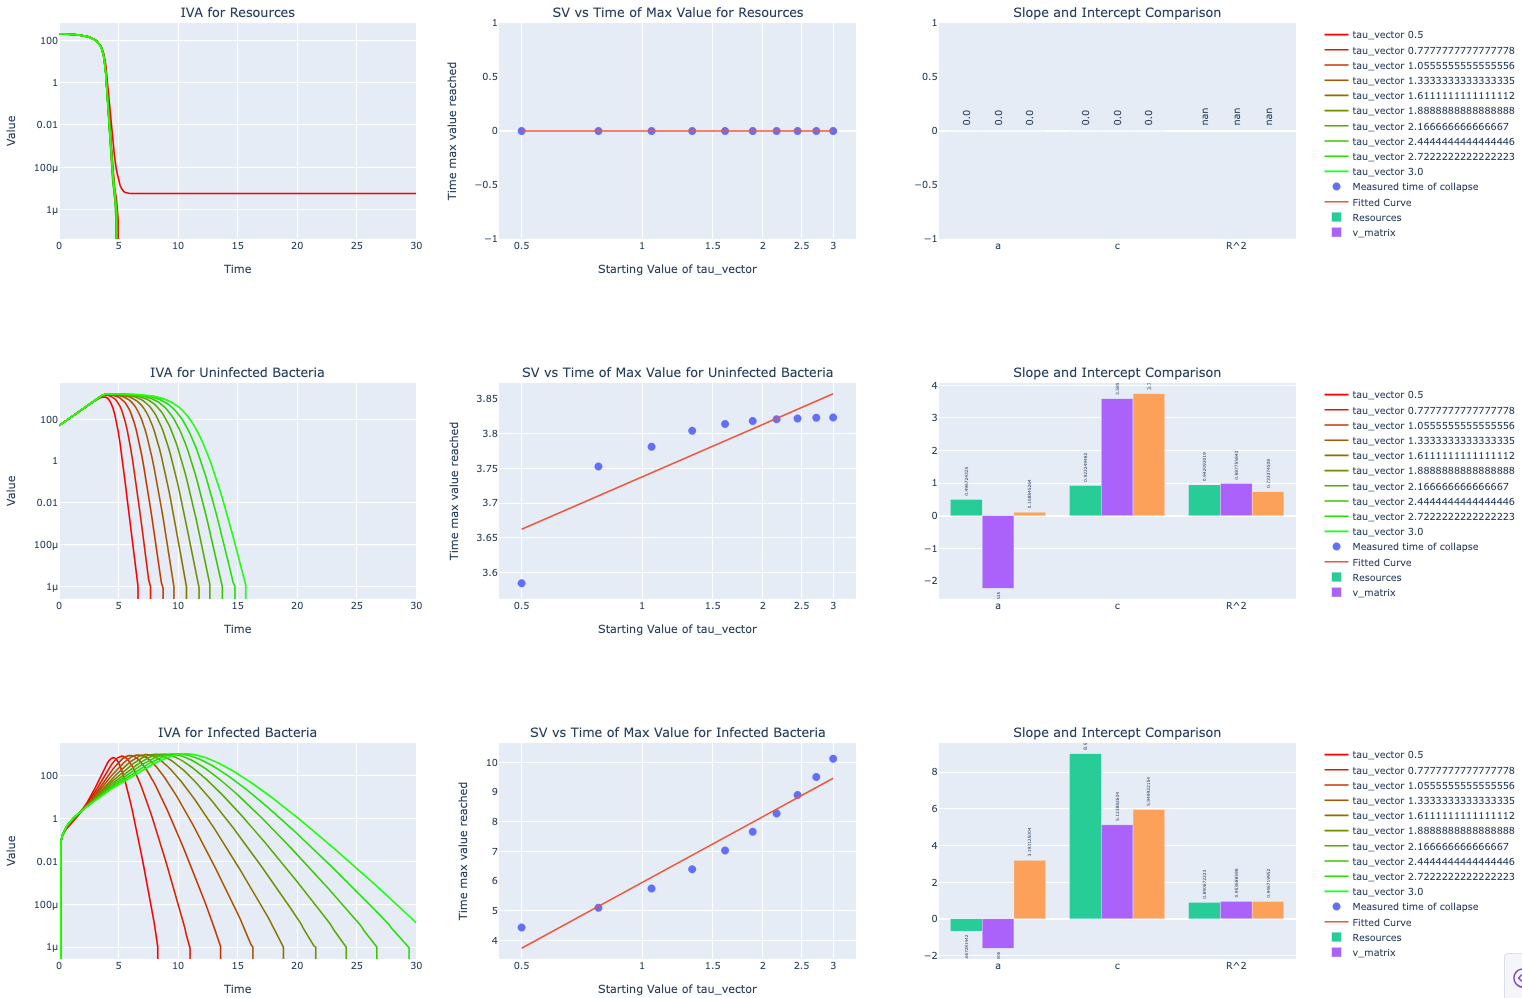
\includegraphics[width=\linewidth]{Screenshots/AdvancedVisualization/initial_value_analysis_run.png}
        \caption{
            An example of an IVA output. 
        }
        \label{fig:ss:av:initial_value_analysis_run}
        \vspace*{\fill}
    \end{subfigure}
    \caption{The IVA settings and output. }
\end{figure}

\begin{figure}[]
    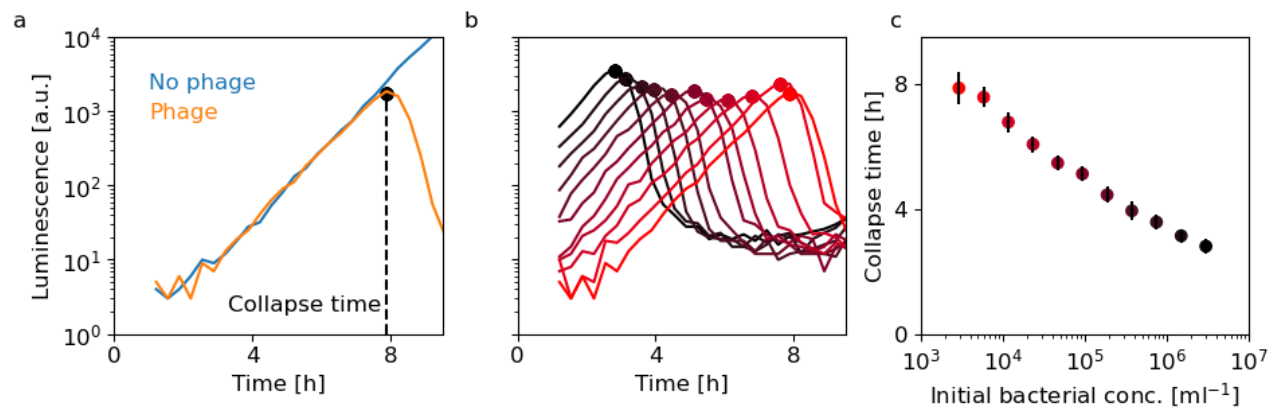
\includegraphics[width=1\textwidth]{Plots/Sourced/Mulla.png}
    \centering
    \caption{
        Phage-induced bacterial population collapse is limited by phage-bacteria adsorption. 
        a) Exemplary growth curve of \text{E. coli} in the absence and presence of a phage (Bas04), measured by bioluminescence. 
        b) Growth curves measured at different initial bacterial concentrations $b_0$ ($3\times10^3 - 3\times 10^6 ml^{-1}$ from red to black; colors as in c) at a fixed multiplicity of infection (MOI, i.e. phage-to-bacteria ratio) of 0.4. 
        c) Collapse times from b); the observed logarithmic decrease (Pearson's $\rho=0.995, p=10^{-10})$ suggests that the phage-amplification kinetics is adsorption-limited. 
        Error bars show standard errors from bootstrapping the growth curves.
        Figure and caption sourced from \citet{mullaExtremeDiversityPhage2024}. 
    }
    \label{fig:sourced:Mulla}
\end{figure}

\paragraph{Phase Portrait}
\label{sec:phase_portrait}
The phase portrait plot enables users to analyze how a phage, bacterium, or resource population evolves in relation to one another.
Phase portraits indicate how one population increases while the other decreases and vice versa.
Steady states can be identified and classified as either stable, unstable, or saddle points. 
It is also possible to visually identify attractor and repeller points by observing where the population values tend to trend. 
By comparing different starting points, it is possible to see if the system is chaotic or not.
\Cref{fig:ss:av:phase_portrait_settings} and \Cref{fig:ss:av:phase_portrait_run} show the phase portrait setup and sample output. 

\begin{figure}[h!]
    \centering
    \begin{subfigure}{0.49\linewidth}
        \centering
        \captionsetup{width=1\linewidth}
        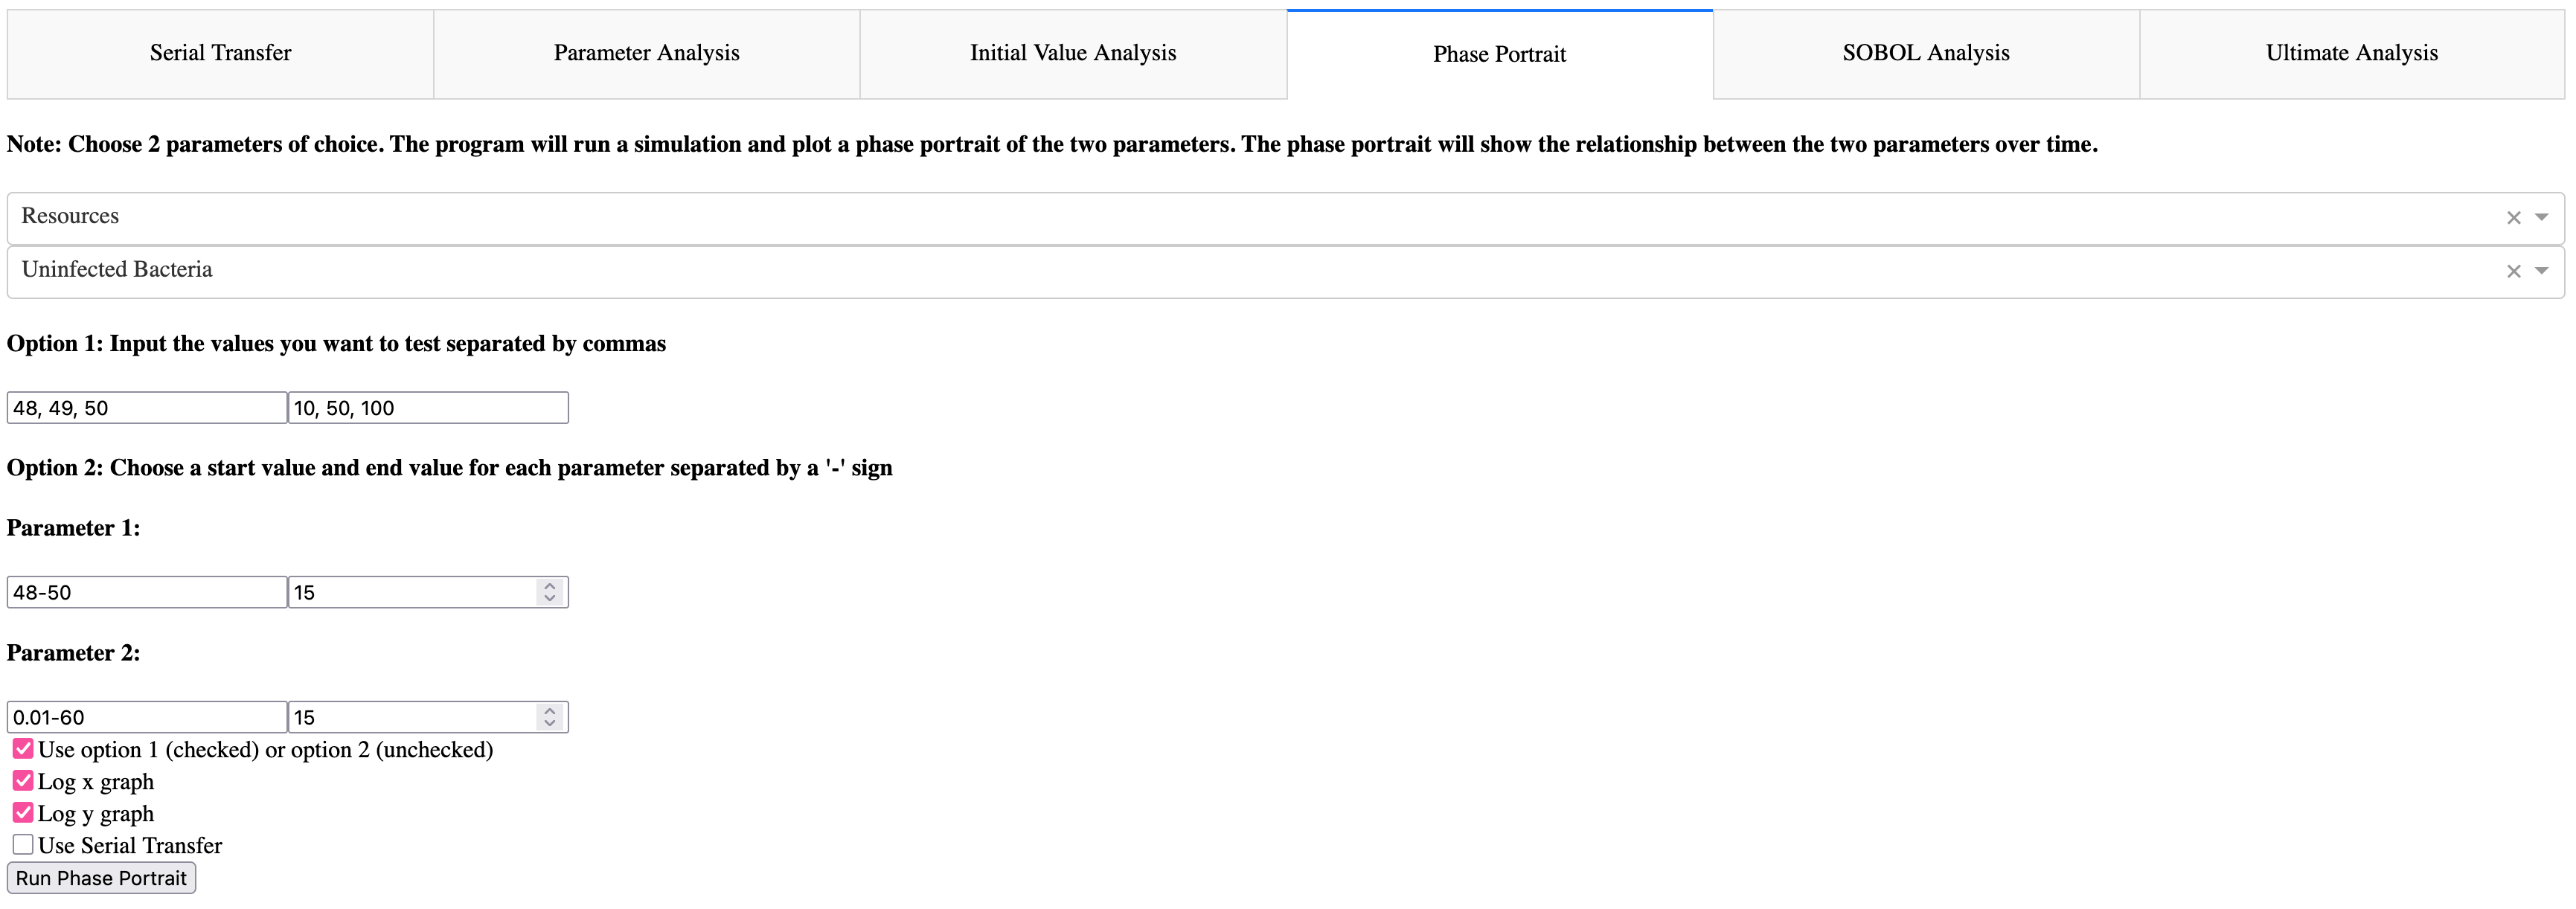
\includegraphics[width=\linewidth]{Screenshots/AdvancedVisualization/phase_portrait_settings.png}
        \caption{
            The user can select two starting values for the IC. 
            However, they cannot choose vector, matrix, or environment settings, as the plot displays the development of phage, bacteria, or resource populations against other phage, bacteria, or resource populations.
            As typical, the user can select their own values or auto-generate values between two values, as well as use an ST option.
            There is also an option to take the logarithm of the x and/or y-axis. 
        }
        \label{fig:ss:av:phase_portrait_settings}
    \end{subfigure}
    \hfill
    \begin{subfigure}{0.49\linewidth}
        \centering
        \captionsetup{width=1\linewidth}
        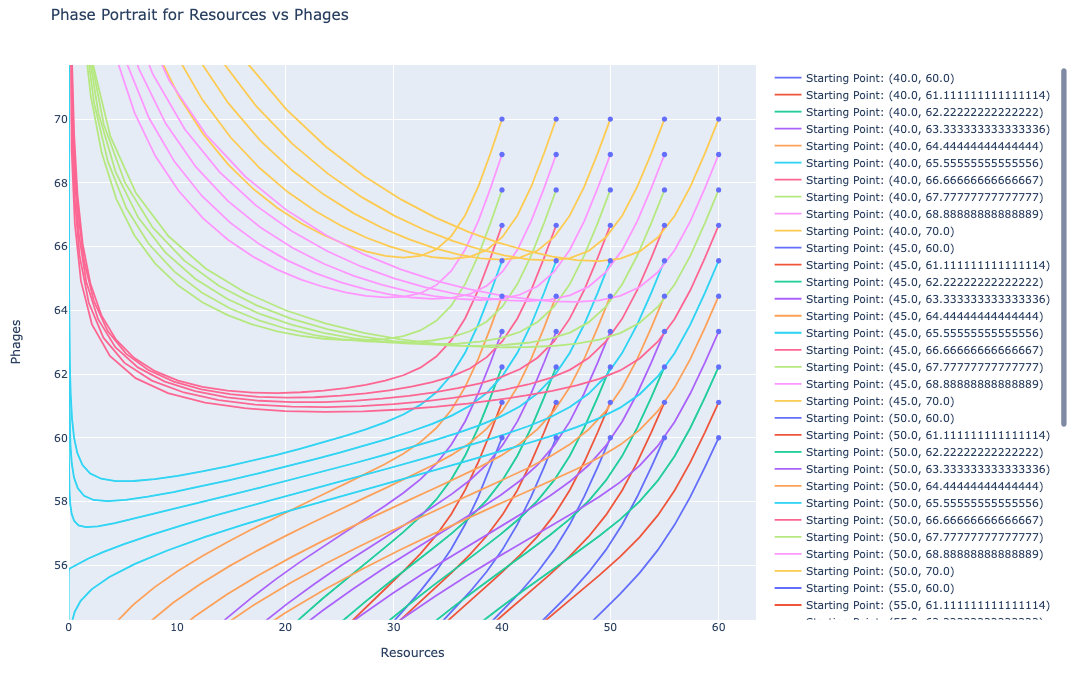
\includegraphics[width=\linewidth]{Screenshots/AdvancedVisualization/phase_portrait_run.png}
        \caption{
            An example phase portrait run. 
        }
        \label{fig:ss:av:phase_portrait_run}
    \end{subfigure}
    \caption{Phase portrait settings and output. }
\end{figure}

\paragraph{Sobol Sensitivity Analysis}
\label{sec:Sobol_sensitivity_analysis}
It is essential to understand how a change in parameter value impacts the output of a model. 
Models will have parameters that are more important and have a greater impact on the model's output than other parameters. 

Sobol analysis \cite{sobolGlobalSensitivityIndices2001}, a variance-based sensitivity analysis, is a method that allows a user to quantify the importance of input parameters on a measured aspect of the output by changing the input parameter values of the model and measuring the resulting change in model output.
Sobol can only measure a single univariate model output, for example, the final population value, the smallest or largest value reached, the time at which the largest value was reached, or any other univariate output. 
Sobol quantifies the variance in the output that can be attributed to a specific parameter and measures the effects of global/total ($ST$), first-order ($S1$), and second-order sensitivity ($S2$). 

First order $Si$, or local sensitivity, is the measurement of the effect that parameter $i$ has on the variance of the output. 
The second order is the measurement of the interaction between parameter $i$ and parameter $j$ and how this interaction contributes to the output variance. 
Etc. for third order and higher. 
Global, also known as total sensitivity, is the sum of all interactions. 
If $ST_i \gg S1_i$, then parameter $i$ depends on higher-order interactions with other parameters, while when $ST_i \approx S1_i$, then $i$ does not interact much with and depend on other parameters.
$ST_i \geq S1_i$ and $ST_i$ can be greater than 1, while $S1_i \leq 1$. 

When a model is treated as a black-box model, the model acts as a function $Y=f(X)$, where $X$ is an input vector of $d$ parameter values, and $Y$ is a univariate model output.
The first-order sensitivity measures the output variance resulting from the primary effect of parameter $X_i$.
Measuring the effect of varying $X_i$ averaged over other input parameters and standardized to provide a fractional contribution to the overall output variance.
The following equation describes the first-order sensitivity. 
\[
 S1_i = \frac{V_i}{\textit{Var}(Y)}
\] where $V_i = \textit{Var}_{X_i}(\mathbb{E}_{X_{\sim i}}[Y|X_i])$ and where $X_{\sim i}$ represents all the parameters that are not $X_i$.
All parameters are summarized in \Cref{tab:appendixA:parameter_table_Sobol}

The second-order index measures the impact of the interaction between input $X_i$ and $X_j$. 
For many inputs, this becomes unwieldy to analyze.
The global sensitivity is used to analyze the global sensitivity without evaluating $2^d-1$ indices. 
It measures the contribution to the output variance of $X_i$, including all variance due to $ X_i$'s interaction with other variables.
\[
 S1_i = \frac{\mathbb{E}_{X_{\sim i}}[\textit{Var}_{X_i}(Y|X_{\sim i}))}{\textit{Var}(Y)} = 1 - \frac{\textit{Var}_{X_i}(\mathbb{E}_{X_i}[Y|X_{\sim i}])}{\textit{Var}(Y)}
\]

Sobol accepts a list of parameter names and an interval of values to sample from, which the user can input in the Sobol settings tab, \Cref{fig:ss:av:Sobol_analysis_settings}. 
If you do not specify any values, the simulation excludes the parameter and uses the default value instead.
The user then needs to select the number of samples to run, using the formula $2^x$, where $x$ is the number they input, and $2^x$ is the number of samples that Sobol will create and run.
The larger $x$ is, the more accurate the Sobol analysis results will be, but the more simulations we will need to run. 
If the second order is not chosen, we run the model $N(D+2)$ times with the randomly sampled input values. 
If the user wants to analyze the second-order interactions, then the model will run the system $N(2D+2)$ times, where $N$ is a multiple of 2, and $D$ is the number of input parameters.
Due to the randomness of the sampling method, the user can, but does not need to, submit a seed value. 

\Cref{fig:ss:av:Sobol_analysis_run} shows a sample Sobol output. 
The global and first-order sensitivities are displayed side by side, with each sub-row in a plot representing a specific entity type. 
We can see the proportion of the global and local sensitivity for each entity type and each parameter.

Upon completion of a Sobol analysis, the original simulation data is saved to the disk as a \textit{.pickle} file so that the user can reuse the data and run their own Sobol analyses. 

\begin{figure}[h!]
    \centering
    \begin{subfigure}{0.49\linewidth}
        \centering
        \captionsetup{width=1\linewidth}
        \includegraphics[width=\linewidth]{Screenshots/AdvancedVisualization/Sobol_analysis_settings.png}
        \caption{
            The Sobol settings tab. 
        }
        \label{fig:ss:av:Sobol_analysis_settings}
    \end{subfigure}
    \hfill
    \begin{subfigure}{0.49\linewidth}
        \centering
        \captionsetup{width=1\linewidth}
        \includegraphics[width=\linewidth]{Screenshots/AdvancedVisualization/Sobol_analysis_run.png}
        \caption{
            Sobol's expected output. 
        }
        \label{fig:ss:av:Sobol_analysis_run}
    \end{subfigure}
    \caption{Sobol variance analysis settings and output. }
\end{figure}

\paragraph{Ultimate Analysis}
\label{sec:ultimate_analysis}
Creating a dashboard that can accommodate various inputs is challenging. 
Predicting the type of plots that a user might be interested in and the type of behavior they want to analyze is impossible to predict. 
The Ultimate Analysis section does not produce any visualizations or analysis; instead, it allows the user to define which ICs and parameter values they want to simulate (\Cref{fig:ss:av:ultimate_analysis_settings}).
The solver will iterate over every possible parameter input and save the results in a \textit{.parquet} file..

Using Dask and the saved \textit{.parquet} file, the user can query for specific runs, for example, runs where a parameter value was greater than 0.05, and use the simulation data to create their own plots.
\begin{figure}
    \centering
    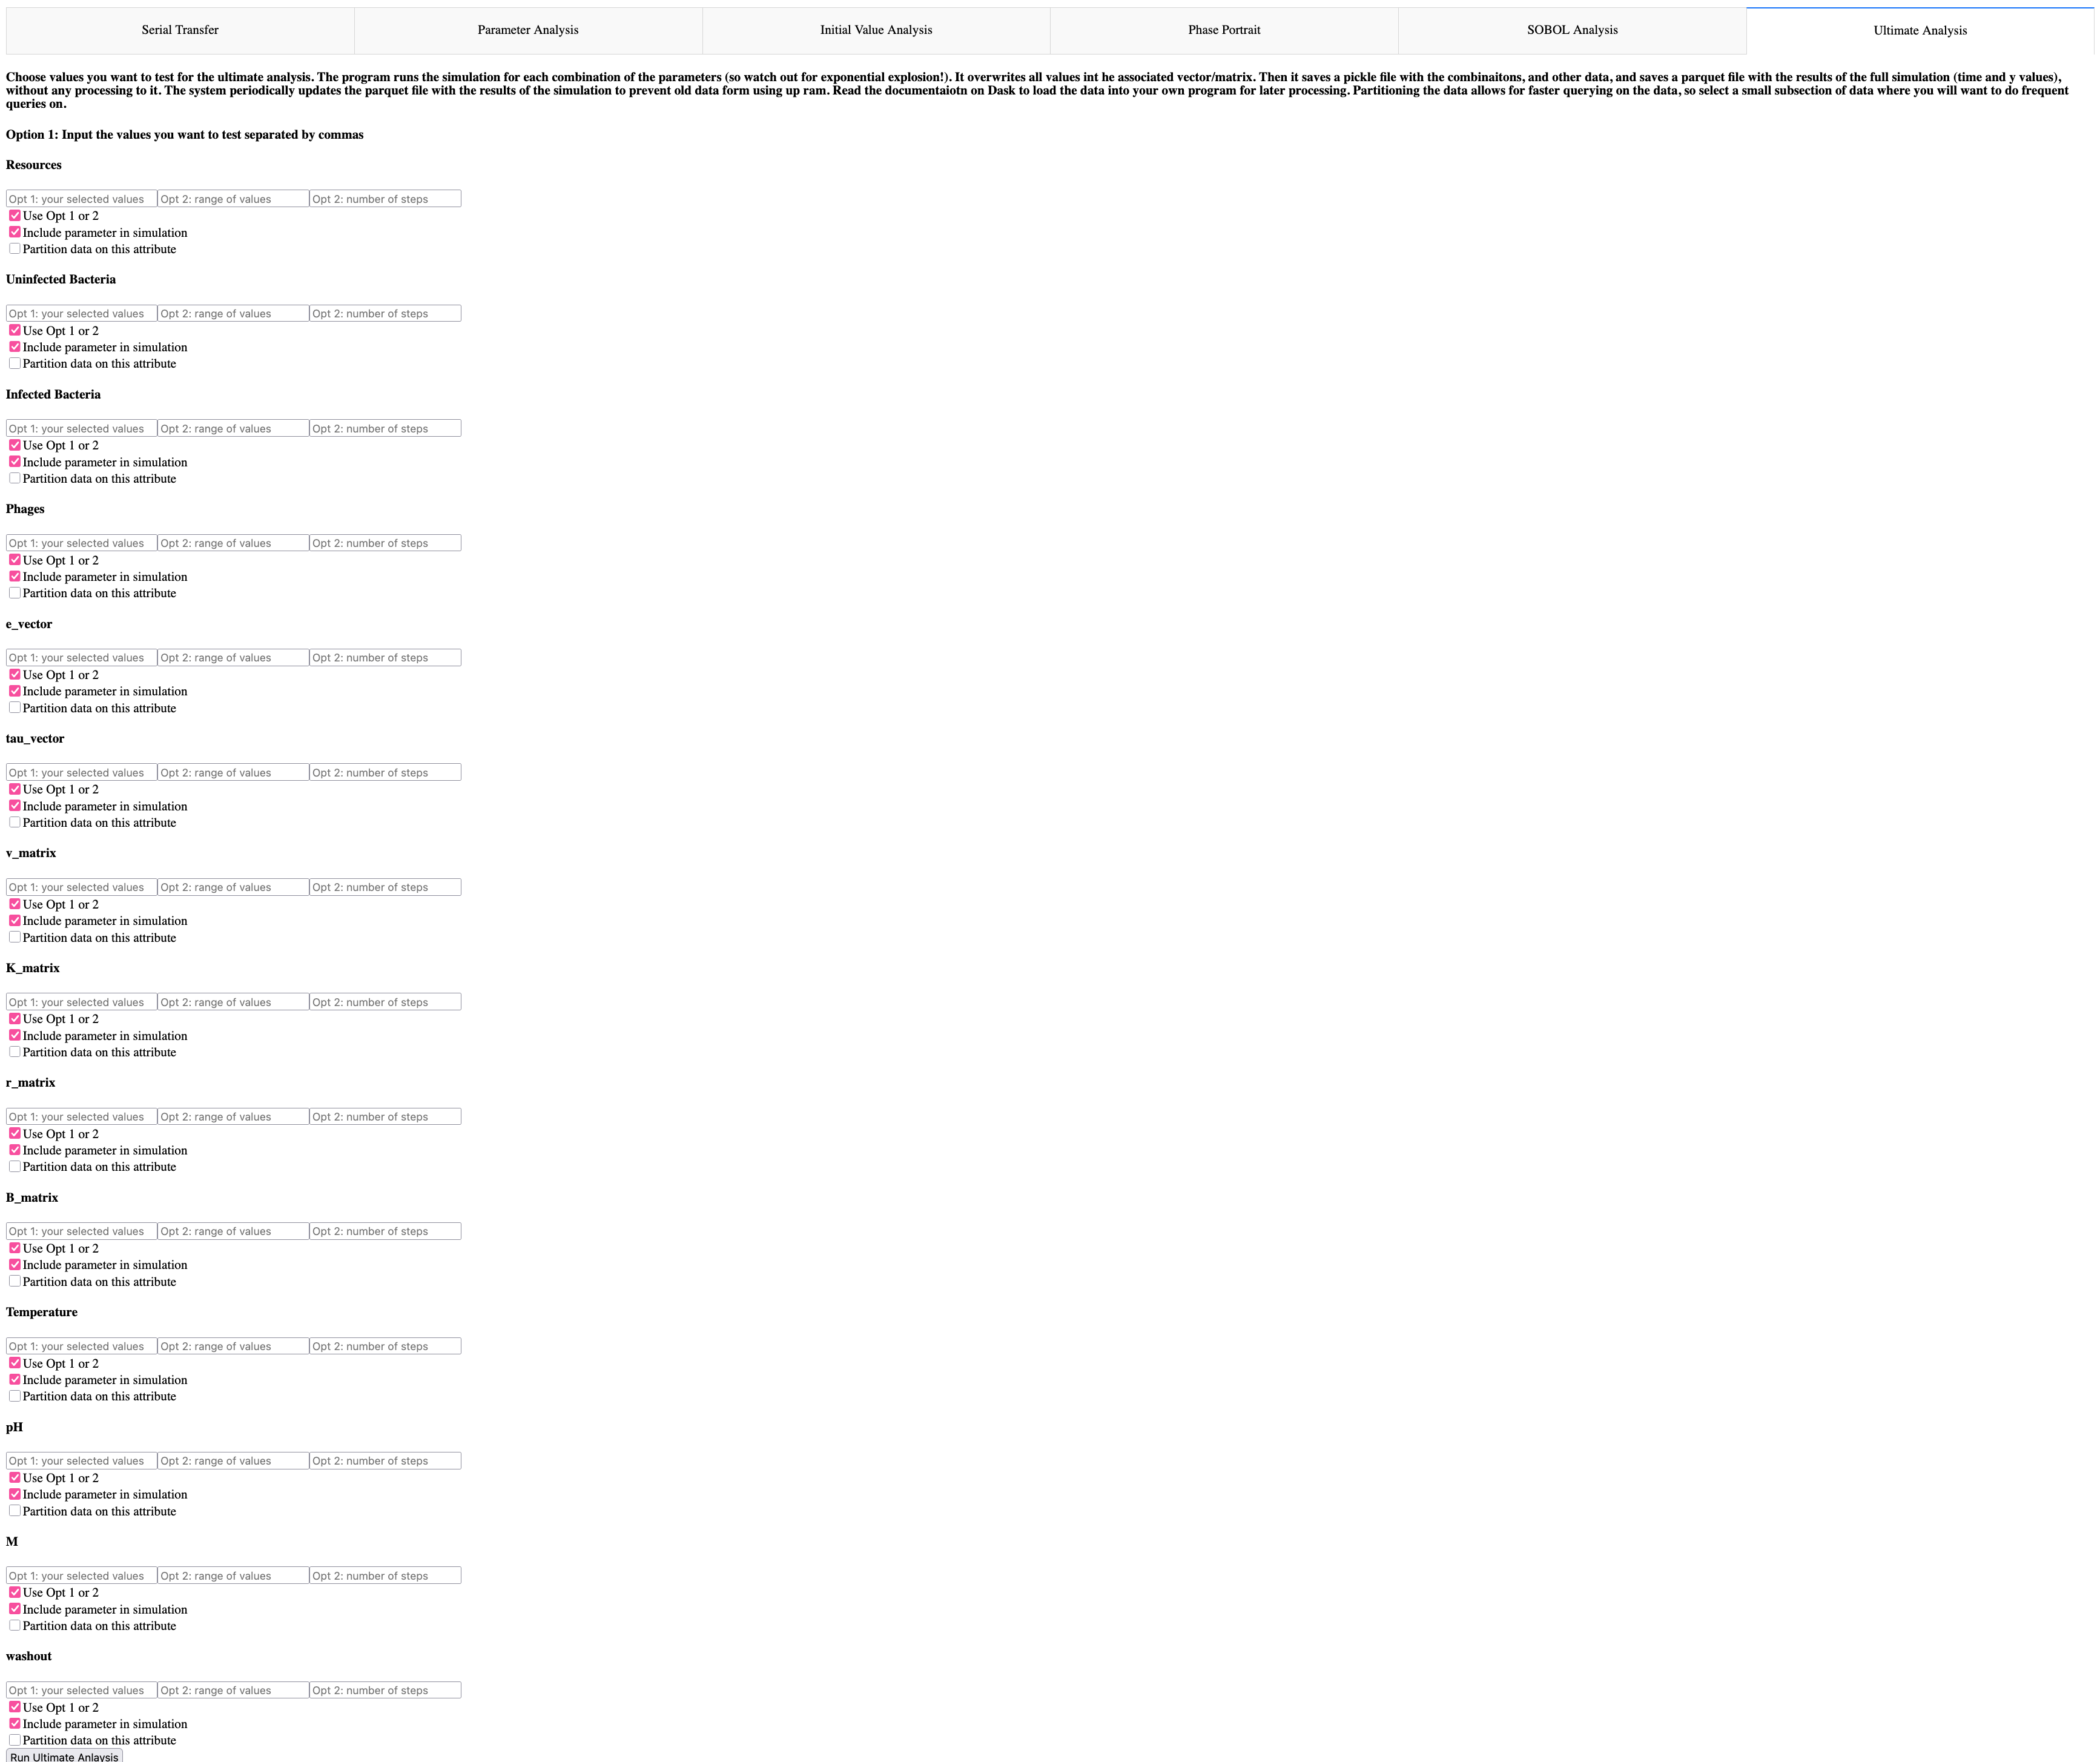
\includegraphics[width=1\linewidth]{Screenshots/AdvancedVisualization/ultimate_analysis_settings.png}
    \caption{
        The Ultimate Analysis setup tab. 
    }
    \label{fig:ss:av:ultimate_analysis_settings}
\end{figure}

\subsection{Custom Visualizations and Analyses} 
\label{sec:custom_visualizations_and_framework}
The final part, an optional step, allows the user to define the parameters they want to simulate and download the simulation results. 
The user can use this data to create their own custom visualizations without having to rerun the simulations, especially if there are many simulations. 
The data can be further processed and visualized as desired by the user. 

As the dashboard cannot create a graph for every situation or be easily adapted to analyze every situation, \Cref{sec:ultimate_analysis} can be used to run and download the simulation data to the disk to create your own custom visualizations later. 

\section{Software Used and Packages}
I created the program with Python \cite{Python} and extensively use various packages, ranging from standard scientific packages such as NumPy \cite{NumPy} and SciPy to more niche packages, including pickle and SALib \cite{iwanagaSALib20Advancing2022, hermanSALibOpensourcePython2017}.

The graphical tool utilizes Tkinter as the front end, handling user inputs, while NetworkX \cite{hagbergExploringNetworkStructure2008} stores the graph and contains the attribute data of the edges and nodes. 
The GUI tool displays a generated graphical representation of the graph. 
The creation of the picture utilizes Matplotlib \cite{Matplotlib} to generate the graph figure. 

The simulation framework, the backend of the modeling, makes extensive usage of SciPy's \textit{solve\_ivp()} to create the ODE data. 
It also uses NetworkX to load the graph and parameter values. 

The visualization component heavily utilizes Dash and Plotly. 
Dash hosts the web server and displays the HTML and visualizations while handling input and output. 
Upon choosing parameter values and clicking “Submit”, Dash registers the activity and calls the function registered to the button, sending data such as parameter values and options, like “log x-axis” to the backend server. 
In the backend, various inputs are handled, such as converting the input string \textit{“0.05, 0.1, 0.15, 0.2”} into an iterable list \textit{[0.05, 0.1, 0.15, 0.2]} that the simulation framework can iterate over to vary the parameter value. 

If there are many simulations to run, an intermediate call executes Joblib, a parallel computing program, as seen in \Cref{sec:ultimate_analysis} and \Cref{sec:Sobol_sensitivity_analysis}. 
Joblib parallelizes computations across multiple CPUs to speed up computation time. 
The ultimate analysis uses Pandas to write the data to a \textit{.parquet} file. 
Pandas Parquet offers efficient data compression, efficient memory usage, and, when combined with Dask, efficient querying functionalities in a DataFrame format that many data scientists are familiar with. 

Sobol uses the SALib library to sample and analyze the parameter input. 
Both ultimate analysis and Sobol save a \textit{.pickle} file containing a dictionary with the parameter values tested, setting values, and other important information regarding the simulation. 

\Cref{sec:initial_value_analysis} uses SciPy's \textit{curve\_fit()} function to curve fit the points in the middle plot (\Cref{fig:ss:av:initial_value_analysis_run}). 

Other packages used in the project include collections, copy, warnings, itertools, os, datetime, json, gc, and time. 